% Compilador en Overleaf: pdfLaTeX (el que viene por defecto)
% Manual: Instrumentos Integrados
%         Entorno: Instrumentos Digitales (PFD / MFD) — 7mo año, Técnico/a en Aviónica
\documentclass[11pt,a4paper,oneside]{article}
\usepackage[T1]{fontenc}
\usepackage[utf8]{inputenc}
\IfFileExists{spanish.ldf}{\usepackage[spanish,es-noshorthands]{babel}}{}
\usepackage{lmodern} % tipografía estándar de LaTeX (Computer Modern)
\usepackage[a4paper,top=3cm,bottom=2.5cm,left=2.5cm,right=2cm,headheight=15pt,footskip=1.1cm]{geometry}
\usepackage{graphicx}
\usepackage{tikz}
\usetikzlibrary{arrows.meta,positioning,shapes.geometric,decorations.pathmorphing,calc}
\usepackage{xcolor}
\usepackage{enumitem}
\usepackage{fancyhdr}
\usepackage{microtype}
\usepackage{array}
\usepackage{titlesec}
\usepackage[most]{tcolorbox}

% ---------- Formato general
\setlength{\parindent}{0pt}
\setlength{\parskip}{4pt}
\setlist[itemize]{itemsep=1pt,topsep=2pt,parsep=0pt}
\setlist[enumerate]{itemsep=1pt,topsep=2pt,parsep=0pt}
\renewcommand{\arraystretch}{1.15}
\newtcolorbox{recuadro}{enhanced,breakable,colback=white,colframe=black,
  boxrule=0.6pt,arc=0pt,left=5pt,right=5pt,top=3pt,bottom=3pt}
\titleformat{\section}{\large\bfseries\centering}{}{0pt}{}
\titleformat{\subsection}{\large\bfseries\itshape\centering}{}{0pt}{\underline}
\titleformat{\subsubsection}{\normalsize\bfseries}{}{0pt}{}
\titlespacing*{\section}{0pt}{14pt}{8pt}
\titlespacing*{\subsection}{0pt}{12pt}{6pt}
\titlespacing*{\subsubsection}{0pt}{10pt}{3pt}
\titlespacing*{\paragraph}{0pt}{6pt}{0.6em}
\newcommand{\casilla}{\raisebox{-0.12em}{\tikz\draw[thick] (0,0) rectangle (0.34,0.34);}}

% ---------- Encabezado y pie (mismo diseño que el manual de Emprendimientos)
\definecolor{ppAzul}{rgb}{0.267,0.447,0.769}
\definecolor{ppAzulClaro}{rgb}{0.557,0.667,0.859}
\fancypagestyle{materia}{%
  \fancyhf{}%
  \fancyhead[L]{\color{ppAzul}\bfseries\itshape 7mo Año}%
  \fancyhead[R]{\color{ppAzul}\bfseries\itshape Instrumentos Integrados}%
  \fancyfoot[L]{\small\color{ppAzulClaro}\itshape scicolonejulian@impatrq.com}%
  \fancyfoot[C]{\raisebox{-0.7\height}{
\includegraphics[height=0.8cm]{logos/logo-impa}}}%
  \fancyfoot[R]{\small\color{ppAzulClaro}\itshape\thepage}%
  \renewcommand{\headrule}{{\color{ppAzul}\hrule height 0.5pt}}%
  \renewcommand{\footrule}{{\color{ppAzul}\hrule height 0.5pt}\vspace{2pt}}%
}

\begin{document}
% ============================================================
% Carátula — reemplaza el bloque \begin{titlepage}...\end{titlepage}
% Requiere en el preámbulo: \usepackage{graphicx} y \usepackage{tikz}
% Logos en la carpeta logos/ (logo-impa.pdf y logo-pba.pdf)
% ============================================================
\begin{titlepage}
% Logo PBA en el margen superior derecho (posición absoluta en la hoja)
\begin{tikzpicture}[remember picture,overlay]
  \node[anchor=north east,inner sep=0pt]
    at ([xshift=-1.5cm,yshift=-1.2cm]current page.north east)
    {
\includegraphics[width=9.75cm]{logos/logo-pba}};
\end{tikzpicture}

\centering
\vspace*{2.58cm}
% Títulos superiores del logo IMPA
{\fontsize{20.74}{25}\selectfont\bfseries Escuela de Educación Secundaria Técnica\par}
\vspace{0.2cm}
{\fontsize{20.74}{25}\selectfont\bfseries N° 7 - Quilmes\par}
\vspace{0.5cm}
% Logo IMPA centrado y grande

\includegraphics[width=0.775\linewidth]{logos/logo-impa}\par
\vspace{0.4cm}
% Título inferior del logo IMPA
{\fontsize{20.74}{25}\selectfont\bfseries Taller Regional Quilmes\par}
\vspace{2cm}
\fbox{\parbox{0.8\linewidth}{\centering\vspace{1em}
{\fontsize{24.88}{30}\selectfont\bfseries INSTRUMENTOS\\ INTEGRADOS\par}\vspace{0.6em}
{\fontsize{17.28}{21}\selectfont\bfseries\itshape Entorno: Instrumentos Digitales\\ (PFD / MFD)\par}\vspace{1em}}}\par
\vspace{0.8cm}
% Año / curso
{\fontsize{20.74}{25}\selectfont\bfseries 7mo año\par}
\vfill
{\fontsize{14.4}{17.3}\selectfont\bfseries EDICIÓN\par}
\vspace{0.2cm}
{\fontsize{14.4}{17.3}\selectfont\bfseries CICLO LECTIVO 2026\par}
\end{titlepage}

\pagestyle{materia}
\setcounter{page}{2}
% ============================================================
% PRESENTACIÓN DE LA MATERIA
% ============================================================
\section*{PRESENTACIÓN DE LA MATERIA}
\subsection*{Instrumentos Integrados}

\begin{center}
\small
\begin{tabular}{|p{0.32\linewidth}|p{0.58\linewidth}|}
\hline
\textbf{Escuela} & E.E.S.T. N° 7 ``Taller Regional Quilmes'' (IMPA) \\ \hline
\textbf{Especialidad} & Técnico/a en Aviónica \\ \hline
\textbf{Año} & 7mo año \\ \hline
\textbf{Campo} & Formación Técnico Específica \\ \hline
\textbf{Módulo} & Sistemas de Instrumentos de la Aeronave (Diseño Curricular 2025) \\ \hline
\textbf{Entorno} & Instrumentos Integrados -- Instrumentos Digitales (PFD / MFD) \\ \hline
\textbf{Carga horaria del módulo} & 4 horas semanales -- 144 horas anuales \\ \hline
\textbf{Marco curricular} & Diseño Curricular 2025 de la Educación Secundaria Técnica, Provincia de
Buenos Aires \\ \hline
\textbf{Docente} & Téc. Aviónico Julián Scicolone -- scicolonejulian@impatrq.com \\ \hline
\end{tabular}
\end{center}

% ------------------------------------------------------------
\section*{FUNDAMENTACIÓN}

El Diseño Curricular plantea que, en la atención de las aeronaves, es necesario conocer las
técnicas de \textbf{operación, montaje y mantenimiento de los sistemas de instrumentos
eléctricos, neumáticos, hidráulicos, de navegación e integrados}, y el uso de herramientas de mano
y especiales en prácticas de montaje y desmontaje de sus componentes. Estos sistemas establecen
un \textbf{cuarto nivel de complejidad} en las prácticas de mantenimiento: montaje y desmontaje,
inspección, evaluación del estado general de los componentes electrónicos y la tecnología de los
materiales. Se suman las capacidades de interpretación, organización, planificación y
certificación de los procesos, para trabajar en talleres de aviónica con su documentación, su
herramental específico y sus normas.

Este manual se centra en los \textbf{instrumentos integrados}: las pantallas de vuelo primarias
(\textbf{PFD}) y multifunción (\textbf{MFD}) que reemplazaron a los instrumentos de aguja, desde
los sistemas completos como el \textbf{Garmin G1000} y el \textbf{G5000} hasta los equipos de
reemplazo que hoy se instalan en la aviación general (\textbf{G5, GI 275, G3X Touch, TXi, AXIS,
Aspen}). Y en el oficio que hace posible instalarlos: \textbf{cables, terminales, crimpado,
conectores militares y D-sub, herramientas y ferretería} de la aviónica.

\begin{recuadro}
\textbf{La realidad del trabajo.} En un taller de aviónica de aviación general, gran parte del
trabajo diario es \textbf{modernizar paneles}: sacar instrumentos de vacío y de aguja, instalar
pantallas digitales, armar mazos de cables, crimpar cientos de contactos, configurar los equipos y
probarlos. Un mazo bien hecho funciona durante décadas; un contacto mal crimpado genera una falla
intermitente que nadie encuentra. Esta materia es ese oficio.
\end{recuadro}

% ------------------------------------------------------------
\section*{OBJETIVOS DE APRENDIZAJE}
Según el Diseño Curricular 2025, se espera que las y los estudiantes puedan:
\begin{itemize}
  \item Interpretar el funcionamiento de los componentes electrónicos y de los equipos, sobre la
        base de los principios físicos que regulan su funcionamiento y de la tecnología aplicada.
  \item Planificar y realizar el mantenimiento de los distintos equipos según las normativas
        vigentes y el criterio personal y profesional necesario.
  \item Determinar los métodos y los tiempos necesarios para las tareas de mantenimiento básico.
  \item Confeccionar y completar la documentación técnica de todas las etapas del mantenimiento.
  \item Desenvolverse profesionalmente dentro de un taller de aviónica, priorizando el trabajo
        grupal e interdisciplinario, la seguridad y el seguimiento de las normas vigentes.
  \item Interiorizarse en los avances y desarrollos de las nuevas tecnologías y la innovación
        digital, y su aplicación en el campo.
\end{itemize}

% ------------------------------------------------------------
\section*{ORGANIZACIÓN DEL MANUAL}

\begin{center}
\small
\begin{tabular}{|c|>{\raggedright\arraybackslash}p{0.52\linewidth}|>{\raggedright\arraybackslash}p{0.29\linewidth}|}
\hline
\textbf{Unidad} & \textbf{Contenidos} & \textbf{Contenido del Diseño Curricular} \\ \hline
1 & Del panel analógico a la cabina de cristal: T básica, EFIS, arquitecturas, normas y
certificación. & Clasificación y agrupación de instrumentos; sistemas electrónicos de vuelo \\
\hline
2 & Sensores: pitot-estático, ADC, AHRS, magnetómetro, sensores de motor; buses de datos. & Sistemas
de presión, ADC; actitud, rumbo; indicadores de motor \\ \hline
3 & PFD y MFD: presentación, alertas, banderas, modos reversionarios, instrumentos de reserva. &
Sistemas electrónicos de vuelo y de aviso \\ \hline
4 & Sistemas integrados Garmin G1000 / G1000 NXi y G5000. & Sistemas electrónicos de vuelo \\ \hline
5 & Equipos de reemplazo: G5, GI 275, G3X Touch, G500/G600 TXi, AXIS, Aspen. & Sistemas
electrónicos de vuelo; nuevas tecnologías \\ \hline
6 & Cables aeronáuticos, mazos, blindajes, masas y EWIS. & Instalación y normas: cables \\ \hline
7 & Terminales, empalmes, crimpado y soldadura. & Instalación y normas: pines \\ \hline
8 & Conectores circulares militares y D-sub. & Instalación y normas: pines, cables \\ \hline
9 & Herramientas del taller y ferretería eléctrica y electrónica aplicada. & Herramientas de mano y
especiales \\ \hline
10 & Instalación, configuración y documentación de un panel digital. & Instalación y normas
(tableros, iluminación) \\ \hline
11 & Ensayos, calibración, sistema pitot-estático y diagnóstico de fallas. & Ensayo, mediciones y
calibración; chequeo funcional \\ \hline
TP & Trabajos prácticos de taller. & Prácticas formativas \\ \hline
PI & Proyecto integrador: panel didáctico con su mazo de cables. & Prácticas formativas \\ \hline
\end{tabular}
\end{center}

\paragraph*{Metodología.} Cada unidad combina teoría, documentación real (manuales de instalación
y de mantenimiento de los fabricantes), ejemplos numéricos y actividades. Los \textbf{trabajos
prácticos} se hacen en el banco: crimpado, armado de conectores, mazos, ensayos de continuidad,
configuración y prueba pitot-estática. Cierra con un \textbf{proyecto integrador}: un panel
didáctico completo con su mazo de cables y su documentación.

\paragraph*{Fuentes.} Los datos de cada equipo (números de parte, conexiones, configuraciones) se
toman siempre del \textbf{manual de instalación vigente del fabricante}. Este manual da ejemplos
para aprender; no reemplaza esa documentación.

% ------------------------------------------------------------
\section*{SEGURIDAD EN EL TALLER DE AVIÓNICA}
\begin{recuadro}
\begin{enumerate}
  \item \textbf{Desenergizar} antes de conectar o desconectar equipos: batería desconectada o
        disyuntores abiertos con collar y tarjeta.
  \item \textbf{Descarga electrostática:} pulsera y superficie antiestática para manipular
        pantallas y computadoras; guardarlas en bolsas antiestáticas.
  \item \textbf{Herramientas de corte y pelado:} cuchillas siempre guardadas; nunca pelar cables
        hacia el cuerpo.
  \item \textbf{Pistola de calor y soldador:} superficies calientes; no dejarlos apoyados sobre
        cables ni sobre la mesa.
  \item \textbf{Sistema pitot-estático:} nunca soplar ni aplicar presión o vacío bruscos: se dañan
        los instrumentos y los sensores.
  \item \textbf{Orden y limpieza:} recortes de cable, contactos sueltos y virutas son
        \textbf{FOD}: pueden terminar dentro de un conector o de un equipo.
\end{enumerate}
\end{recuadro}

% ------------------------------------------------------------
\clearpage
\section*{HOJA DE RUTA DEL ESTUDIANTE}
\subsection*{Lo que vas a tener hecho al terminar el año}

\vspace{2pt}
{\small
\renewcommand{\arraystretch}{1.2}
\begin{tabular}{|c|>{\raggedright\arraybackslash}p{0.54\linewidth}|>{\centering\arraybackslash}p{0.08\linewidth}|>{\centering\arraybackslash}p{0.17\linewidth}|}
\hline
\textbf{OK} & \textbf{Logro} & \textbf{Unidad} & \textbf{Firma docente} \\ \hline
\casilla & Identificación de la T básica y de los datos de un PFD y un MFD & 1--3 & \\ \hline
\casilla & Diagrama de bloques de un sistema integrado (sensores, pantallas, buses) & 2--4 & \\
\hline
\casilla & Operación de un PFD y un MFD en simulador o entrenador & 3--4 & \\ \hline
\casilla & Cuadro comparativo de equipos de reemplazo (G5, GI 275, G3X, TXi, AXIS, Aspen) & 5 & \\
\hline
\casilla & Cálculo de sección de cable y caída de tensión & 6 & \\ \hline
\casilla & Crimpado de terminales y empalmes con ensayo de tracción & 7 & \\ \hline
\casilla & Terminación de un blindaje con manguito de soldadura & 7 & \\ \hline
\casilla & Armado de un conector D-sub de alta densidad con contactos crimpados & 8 & \\ \hline
\casilla & Inserción y extracción de contactos en un conector circular MIL-DTL-38999 & 8 & \\ \hline
\casilla & Inventario y uso correcto de las herramientas del taller & 9 & \\ \hline
\casilla & Plano de cableado de una instalación a partir del manual del fabricante & 10 & \\ \hline
\casilla & Mazo de cables armado, identificado y verificado pin a pin & 10 & \\ \hline
\casilla & Configuración y calibración de un equipo (o en modo entrenamiento) & 10 & \\ \hline
\casilla & Ensayo de pérdidas del sistema pitot-estático con banco de prueba & 11 & \\ \hline
\casilla & Diagnóstico de una falla simulada y tarjeta de trabajo completa & 11 & \\ \hline
\casilla & Proyecto integrador: panel didáctico presentado & PI & \\ \hline
\end{tabular}
}

\vspace{8pt}
\noindent Estudiante: \dotfill \quad Curso: \makebox[3cm]{\dotfill}

\vspace{6pt}
\noindent Logros completados: \makebox[1.5cm]{\dotfill} de 16 \hfill Fecha: \makebox[4cm]{\dotfill}
   % Fundamentación, objetivos, organización, seguridad y hoja de ruta
% ============================================================
% UNIDAD 1: DEL PANEL ANALÓGICO A LA CABINA DE CRISTAL
% ============================================================
\clearpage
\section*{UNIDAD 1: LA CABINA DE CRISTAL}
\subsection*{Del panel analógico a los instrumentos integrados}

\begin{recuadro}
\textbf{Objetivo de la unidad:} conocer la clasificación y agrupación de los instrumentos de
vuelo, la evolución hacia los sistemas electrónicos de vuelo (EFIS), las arquitecturas de los
instrumentos integrados y el marco de normas y certificación en el que se instalan.
\end{recuadro}

% ------------------------------------------------------------
\section*{1. LOS INSTRUMENTOS CLÁSICOS Y LA T BÁSICA}

Los instrumentos de una aeronave se clasifican en \textbf{instrumentos de vuelo} (actitud,
velocidad, altitud, rumbo), \textbf{de navegación} (VOR, ILS, GPS, ADF), \textbf{de motor}
(revoluciones, presiones, temperaturas, combustible) y \textbf{de sistemas} (eléctrico,
hidráulico, presurización, tren, flaps).

Durante décadas los instrumentos de vuelo fueron mecánicos o electromecánicos, agrupados en la
\textbf{T básica}: actitud en el centro, velocidad a la izquierda, altitud a la derecha y rumbo
debajo, para que la mirada del piloto recorra siempre el mismo camino. Con el indicador de viraje
y el variómetro se forma el clásico panel de ``seis instrumentos''.

\begin{center}
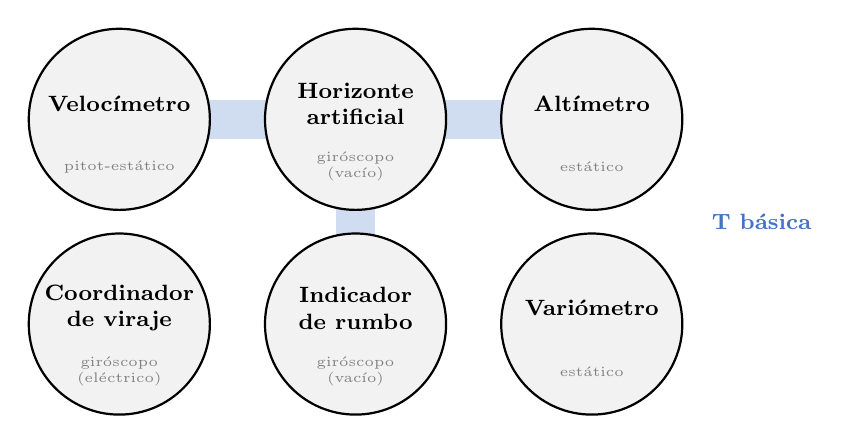
\begin{tikzpicture}[every node/.style={font=\footnotesize, align=center}]
  \draw[ppAzul!25, line width=14pt] (0,2.6) -- (6,2.6);
  \draw[ppAzul!25, line width=14pt] (3,2.6) -- (3,0);
  \draw[thick, fill=gray!10] (0,2.6) circle (1.15);
  \node[font=\footnotesize\bfseries] at (0,2.8) {Velocímetro};
  \node[gray] at (0,2.0) {\tiny pitot-estático};
  \draw[thick, fill=gray!10] (3,2.6) circle (1.15);
  \node[font=\footnotesize\bfseries] at (3,2.8) {Horizonte\\ artificial};
  \node[gray, font=\tiny] at (3,2.0) {giróscopo\\ (vacío)};
  \draw[thick, fill=gray!10] (6,2.6) circle (1.15);
  \node at (6,2.8) {\textbf{Altímetro}};
  \node[gray] at (6,2.0) {\tiny estático};
  \draw[thick, fill=gray!10] (0,0) circle (1.15);
  \node[font=\footnotesize\bfseries] at (0,0.2) {Coordinador\\ de viraje};
  \node[gray, font=\tiny] at (0,-0.6) {giróscopo\\ (eléctrico)};
  \draw[thick, fill=gray!10] (3,0) circle (1.15);
  \node[font=\footnotesize\bfseries] at (3,0.2) {Indicador\\ de rumbo};
  \node[gray, font=\tiny] at (3,-0.6) {giróscopo\\ (vacío)};
  \draw[thick, fill=gray!10] (6,0) circle (1.15);
  \node at (6,0.2) {\textbf{Variómetro}};
  \node[gray] at (6,-0.6) {\tiny estático};
  \node[ppAzul, right] at (7.4,1.3) {\textbf{T básica}};
\end{tikzpicture}
\end{center}

\paragraph*{Problemas del panel analógico.} Instrumentos de vacío con giróscopos que se desgastan;
bombas de vacío que fallan sin aviso; mucho peso y cableado; poca información integrada; cada
instrumento con su propio mantenimiento y calibración.

% ------------------------------------------------------------
\section*{2. LOS SISTEMAS ELECTRÓNICOS DE VUELO (EFIS)}

En los años ochenta los aviones de transporte (Boeing 757/767, Airbus A310) reemplazaron los
instrumentos de actitud y de rumbo por pantallas de tubos de rayos catódicos: el \textbf{EFIS}
(\textit{Electronic Flight Instrument System}). Luego llegaron las pantallas de cristal líquido y la
integración total. En la aviación general, el \textbf{Garmin G1000} (2004) llevó la
\textbf{cabina de cristal} (\textit{glass cockpit}) a los aviones livianos.

\begin{center}
\small
\begin{tabular}{|p{0.18\linewidth}|p{0.70\linewidth}|}
\hline
\textbf{Pantalla} & \textbf{Función} \\ \hline
\textbf{PFD} & \textit{Primary Flight Display}: reúne la T básica en una sola pantalla (actitud,
velocidad, altitud, velocidad vertical, rumbo) más la navegación, el piloto automático y las
alertas. \\ \hline
\textbf{MFD} & \textit{Multi-Function Display}: mapa móvil, motor, tránsito, meteorología, terreno,
cartas, listas de chequeo. \\ \hline
\textbf{ND} & \textit{Navigation Display}: en aviones de transporte, la pantalla de navegación. \\
\hline
\textbf{EICAS / ECAM} & Pantallas de motor y de alertas de la tripulación (Boeing y Airbus). \\
\hline
\textbf{EIS} & \textit{Engine Indication System}: indicación de motor en aviación general. \\
\hline
\end{tabular}
\end{center}

\paragraph*{Ventajas.} Más información, mejor integrada y presentada de forma más intuitiva;
menos peso; mayor confiabilidad (sin giróscopos mecánicos ni bombas de vacío); autodiagnóstico;
actualización por software; menos cableado gracias a los buses de datos.

\paragraph*{Desafíos.} Dependen totalmente del sistema eléctrico; exigen capacitación de pilotos y
técnicos; las bases de datos y el software deben mantenerse actualizados; una falla puede afectar
varias funciones a la vez. Un estudio de la NTSB de 2010 sobre aviones livianos con cabina de
cristal concluyó que la tecnología por sí sola no mejoraba la seguridad si no venía acompañada de
\textbf{capacitación específica}.

% ------------------------------------------------------------
\section*{3. ARQUITECTURAS}

\begin{itemize}
  \item \textbf{Instrumentos autónomos (\textit{standalone}):} una pantalla con sus sensores
        internos o propios reemplaza a uno o dos instrumentos (G5, GI 275, Aspen).
  \item \textbf{Sistema de pantallas con sensores remotos:} las pantallas reciben los datos de un
        ADAHRS (computadora de datos de aire y referencia de actitud) y otros sensores, y se
        comunican con la radio, el GPS y el piloto automático existentes (G3X Touch, G500/G600
        TXi).
  \item \textbf{Sistema totalmente integrado:} pantallas, sensores, radios, transpondedor, audio y
        piloto automático forman un solo sistema conectado por buses de alta velocidad, con
        unidades de procesamiento centrales (G1000, G3000, G5000, y en los aviones de transporte la
        aviónica modular integrada, IMA).
  \item \textbf{Pantalla con radios integradas:} la tendencia más reciente en aviación general es
        que la pantalla incorpore también el navegador GPS, las radios de comunicaciones y
        navegación y el panel de audio, eliminando la columna central de equipos (Garmin AXIS).
\end{itemize}

\paragraph*{Instrumentos de reserva.} Toda cabina de cristal mantiene \textbf{instrumentos de
reserva} (\textit{standby}) independientes, con su propia batería, para volar si fallan las
pantallas principales: antes eran un horizonte, un altímetro y un velocímetro mecánicos; hoy suele
ser un instrumento electrónico (por ejemplo, un G5 o un GI 275).

% ------------------------------------------------------------
\section*{4. NORMAS Y CERTIFICACIÓN}

\begin{center}
\small
\begin{tabular}{|p{0.26\linewidth}|p{0.62\linewidth}|}
\hline
\textbf{Norma o documento} & \textbf{Qué regula} \\ \hline
TSO (\textit{Technical Standard Order}) & Estándar mínimo de desempeño de un equipo (por ejemplo,
TSO-C113 para pantallas multipropósito). \\ \hline
RTCA DO-160 & Ensayos ambientales: temperatura, vibración, humedad, interferencia, rayos. \\
\hline
RTCA DO-178C / DO-254 & Desarrollo del software y del hardware electrónico complejo. \\ \hline
FAA AC 23.1311-1 & Instalación de pantallas electrónicas en aviones de categoría normal:
ubicación, campo visual, colores, alertas. \\ \hline
FAA AC 43.13-1B y 43.13-2 & Prácticas aceptables de mantenimiento, cableado e instalación de
equipos. \\ \hline
STC (certificado tipo suplementario) & Aprobación de una modificación de diseño. Un
\textbf{AML-STC} cubre una lista de modelos de aeronave. \\ \hline
\end{tabular}
\end{center}

\paragraph*{Aeronaves certificadas, experimentales y LSA.} En una aeronave \textbf{certificada}
solo se pueden instalar equipos con aprobación (TSO) y mediante datos aprobados (STC o aprobación
de campo), y la instalación se documenta como alteración ante la autoridad. En las aeronaves
\textbf{experimentales} (de construcción amateur) y \textbf{LSA} hay más libertad y se usan
versiones experimentales de los equipos, más económicas. Por eso muchos fabricantes ofrecen dos
versiones del mismo equipo. En la Argentina, la instalación en una aeronave certificada requiere
que el STC extranjero esté \textbf{convalidado o aceptado por la ANAC} y que la realice un taller
habilitado.

% ------------------------------------------------------------
\section*{5. ACTIVIDADES DE LA UNIDAD}
\begin{enumerate}
  \item Dibujar la T básica e indicar qué sistema alimenta a cada instrumento (pitot, estática,
        vacío, eléctrico).
  \item Comparar una foto de un panel analógico y una de un panel con G1000: ubicar en el PFD cada
        uno de los seis instrumentos clásicos.
  \item Investigar qué aeronaves de la escuela o del aeródromo más cercano tienen cabina de
        cristal y con qué equipos.
  \item Explicar la diferencia entre un instrumento autónomo, un sistema con sensores remotos y un
        sistema integrado, con un ejemplo de cada uno.
  \item Buscar en la lista de modelos (AML) de un STC de Garmin si incluye a un Cessna 150 o un
        Piper PA-28.
\end{enumerate}
       % Unidad 1: del panel analógico a la cabina de cristal
% ============================================================
% UNIDAD 2: SENSORES, ADAHRS Y BUSES DE DATOS
% ============================================================
\clearpage
\section*{UNIDAD 2: SENSORES Y BUSES DE DATOS}
\subsection*{Pitot-estático, ADC, AHRS, sensores de motor y buses de datos}

\begin{recuadro}
\textbf{Objetivo de la unidad:} conocer de dónde obtienen sus datos los instrumentos integrados:
los sistemas de presión y la computadora de datos de aire, los sensores de actitud y rumbo, los
sensores de motor y los buses de datos que los conectan.
\end{recuadro}

% ------------------------------------------------------------
\section*{1. EL SISTEMA PITOT-ESTÁTICO}

\begin{itemize}
  \item \textbf{Toma pitot:} orientada hacia adelante, recibe la \textbf{presión total} (estática
        más dinámica). Tiene calefacción eléctrica para evitar el hielo.
  \item \textbf{Tomas estáticas:} orificios a ras del fuselaje (generalmente una de cada lado,
        interconectadas) que miden la \textbf{presión estática} del aire.
  \item \textbf{Drenajes:} puntos bajos de las líneas para eliminar el agua.
  \item \textbf{Fuente estática alternativa:} en caso de obstrucción, toma la presión del interior
        de la cabina.
\end{itemize}

\begin{center}
\small
\begin{tabular}{|p{0.26\linewidth}|p{0.22\linewidth}|p{0.40\linewidth}|}
\hline
\textbf{Dato} & \textbf{Presiones usadas} & \textbf{Principio} \\ \hline
Altitud de presión & Estática & La presión disminuye con la altura (atmósfera estándar: 1013,25
hPa, 29,92 inHg al nivel del mar). \\ \hline
Altitud indicada & Estática + ajuste QNH & Corrige por la presión del día. \\ \hline
Velocidad indicada (IAS) & Total -- estática & Presión dinámica $q = \frac{1}{2}\rho v^2$. \\ \hline
Velocidad vertical & Variación de la estática & Ritmo de cambio de la presión. \\ \hline
Mach & Total y estática & Relación entre ambas. \\ \hline
\end{tabular}
\end{center}

% ------------------------------------------------------------
\section*{2. LA COMPUTADORA DE DATOS DE AIRE (ADC)}

La \textbf{ADC} recibe las presiones pitot y estática en \textbf{transductores de presión}
(sensores piezorresistivos o de silicio resonante) y la temperatura exterior desde una
\textbf{sonda de temperatura} (OAT o TAT). Calcula:
\begin{itemize}
  \item Altitud de presión y altitud barométrica corregida.
  \item Velocidad indicada (IAS), calibrada (CAS) y verdadera (TAS, corregida por densidad).
  \item Número de Mach y velocidad vertical.
  \item Temperatura del aire exterior y densidad de altitud.
  \item Altitud codificada para el \textbf{transpondedor} (modo C/S).
\end{itemize}
Envía los resultados por un bus de datos a las pantallas, al transpondedor, al piloto automático y
al GPS. Ventaja: un solo par de líneas de pitot y estática y un solo sensor alimentan a todos los
sistemas.

% ------------------------------------------------------------
\section*{3. ACTITUD Y RUMBO: EL AHRS}

El \textbf{AHRS} (\textit{Attitude and Heading Reference System}) reemplaza a los giróscopos
mecánicos.
\begin{itemize}
  \item \textbf{Giróscopos MEMS:} sensores microelectromecánicos de silicio que miden la velocidad
        de rotación en los tres ejes.
  \item \textbf{Acelerómetros MEMS:} miden las aceleraciones en los tres ejes (incluida la
        gravedad, que da la referencia de ``abajo'').
  \item \textbf{Magnetómetro:} mide el campo magnético terrestre en tres ejes para obtener el
        rumbo. Se instala \textbf{lejos de materiales ferrosos y de cables con corriente} (en un
        ala o en la cola), porque cualquier campo magnético cercano altera la lectura.
  \item \textbf{Ayuda de datos de aire y GPS:} el AHRS usa la velocidad verdadera y la posición GPS
        para corregir los errores de los acelerómetros en virajes y aceleraciones.
\end{itemize}
Un procesador combina todos los datos con filtros (por ejemplo, el filtro de Kalman) y entrega
cabeceo, alabeo, rumbo, velocidad de giro y aceleraciones. Cuando el ADC y el AHRS están en una
misma unidad se llama \textbf{ADAHRS}.

\paragraph*{Comparación con los sistemas inerciales.} Los aviones de transporte usan
\textbf{IRS}/\textbf{ADIRU} con giróscopos láser o de fibra óptica, de mucha mayor precisión, que
además calculan posición. El AHRS de aviación general es más económico y depende de la ayuda del
GPS y de los datos de aire.

\begin{recuadro}
\textbf{Puntos de instalación que el técnico debe cuidar.} El AHRS se monta \textbf{rígido y
alineado} con los ejes de la aeronave (se calibra el cabeceo y el alabeo con la aeronave nivelada).
El magnetómetro se calibra girando la aeronave en distintos rumbos sobre una rosa de los vientos o
siguiendo el procedimiento del fabricante. Cualquier cambio posterior cerca del magnetómetro (un
cable nuevo, una luz estroboscópica, una pieza de acero) obliga a verificarlo.
\end{recuadro}

% ------------------------------------------------------------
\section*{4. SENSORES DE MOTOR Y DE SISTEMAS}

Los sistemas integrados reciben los datos del motor a través de una \textbf{unidad de adquisición}
(por ejemplo, GEA en Garmin) que digitaliza las señales de los sensores:
\begin{center}
\small
\begin{tabular}{|p{0.28\linewidth}|p{0.30\linewidth}|p{0.30\linewidth}|}
\hline
\textbf{Parámetro} & \textbf{Sensor} & \textbf{Señal} \\ \hline
EGT y CHT (temperatura de gases y de cilindros) & Termocuplas tipo K o J & Milivolts \\ \hline
Temperatura de aceite y de aire & Resistencias variables (RTD, termistores) & Resistencia \\ \hline
Presión de aceite, combustible y admisión & Transductores de presión & Tensión (0,5 a 4,5 V) o
corriente \\ \hline
Flujo de combustible & Turbina con sensor óptico o magnético & Pulsos \\ \hline
RPM & Captor magnético o de efecto Hall, o señal de los magnetos & Pulsos \\ \hline
Cantidad de combustible & Flotante resistivo o sonda capacitiva & Resistencia o frecuencia \\ \hline
Corriente eléctrica & Shunt o sensor de efecto Hall & Milivolts \\ \hline
Posición de flaps y compensadores & Potenciómetros & Tensión \\ \hline
\end{tabular}
\end{center}
Cada sensor se configura en el sistema: tipo, rango, marcas de color de los arcos (verde, amarillo,
rojo) según el manual de vuelo y los límites del motor, y la calibración (por ejemplo, la curva de
los tanques de combustible).

% ------------------------------------------------------------
\section*{5. LOS BUSES DE DATOS}

\begin{center}
\small
\begin{tabular}{|p{0.18\linewidth}|p{0.40\linewidth}|p{0.30\linewidth}|}
\hline
\textbf{Bus} & \textbf{Características} & \textbf{Uso típico} \\ \hline
ARINC 429 & Unidireccional, un transmisor y hasta 20 receptores; palabras de 32 bits con etiqueta;
12,5 o 100 kbit/s; par trenzado blindado. & Interconexión con GPS, radios, piloto automático,
equipos de otros fabricantes \\ \hline
RS-232 / RS-422 & Serie, punto a punto; RS-422 diferencial, más inmune al ruido. & Transpondedor,
datos de GPS, configuración \\ \hline
CAN & Bus multipunto diferencial, robusto, con terminaciones de 120 $\Omega$ en los extremos. &
Red de sensores y pantallas (por ejemplo, G3X Touch) \\ \hline
Ethernet (HSDB) & Alta velocidad entre unidades. & Red interna del G1000 y otros sistemas
integrados \\ \hline
ARINC 664 (AFDX) & Ethernet determinística con redundancia. & Aviones de transporte modernos
(A380, B787) \\ \hline
Discretas y analógicas & Señales de encendido/apagado (masa o abierto) y tensiones. & Avisos,
selecciones, sensores \\ \hline
\end{tabular}
\end{center}

\paragraph*{Para el instalador.} Cada bus tiene sus reglas de cableado: pares trenzados y
blindados, impedancia, terminaciones, longitud máxima y forma de conectar los blindajes a masa.
Un ARINC 429 con los cables A y B invertidos o un bus CAN sin su resistencia de terminación son
fallas típicas de instalación.

% ------------------------------------------------------------
\section*{6. ACTIVIDADES DE LA UNIDAD}
\begin{enumerate}
  \item Dibujar el sistema pitot-estático de una aeronave liviana con ADC e indicar qué sistemas
        reciben sus datos.
  \item Con un sensor de presión y un microcontrolador, calcular la altitud de presión con la
        fórmula de la atmósfera estándar y compararla con un altímetro.
  \item Con un módulo de giróscopos y acelerómetros MEMS (tipo MPU-6050 o similar), mostrar en la
        computadora el cabeceo y el alabeo, y observar la deriva del giróscopo sin corrección.
  \item Calcular cuántos milivolts entrega una termocupla tipo K con una diferencia de 400 $^\circ$C
        (aproximadamente 41 $\mu$V/$^\circ$C).
  \item Decodificar una palabra ARINC 429 dada en binario: etiqueta, SDI, datos, SSM y paridad.
\end{enumerate}
    % Unidad 2: sensores, ADAHRS, motor y buses de datos
% ============================================================
% UNIDAD 3: PFD Y MFD
% ============================================================
\clearpage
\section*{UNIDAD 3: EL PFD Y EL MFD}
\subsection*{Presentación de datos, alertas, banderas y modos reversionarios}

\begin{recuadro}
\textbf{Objetivo de la unidad:} interpretar la información que presentan el PFD y el MFD, sus
alertas y sus indicaciones de falla, y conocer los modos reversionarios y los instrumentos de
reserva, desde el punto de vista del técnico que debe verificarlos.
\end{recuadro}

% ------------------------------------------------------------
\section*{1. EL PFD}

\begin{center}
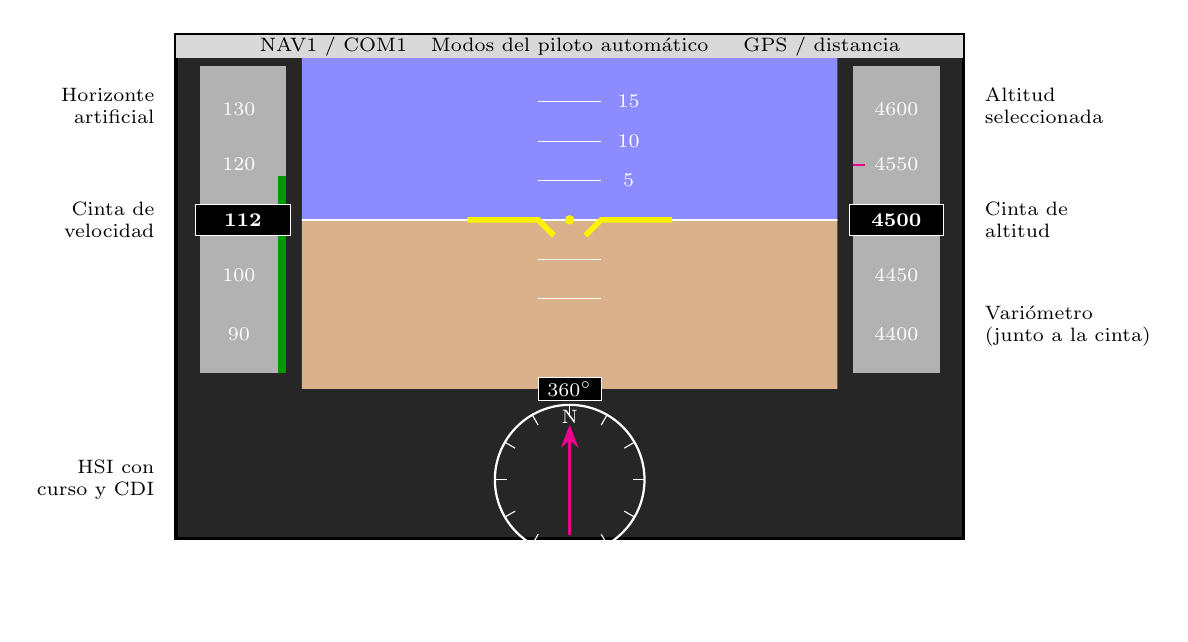
\begin{tikzpicture}[every node/.style={font=\scriptsize}]
  % marco
  \draw[very thick, fill=black!85] (0,0) rectangle (10,6.4);
  % horizonte
  \begin{scope}
    \clip (1.6,1.9) rectangle (8.4,6.2);
    \fill[blue!45] (0,4.05) rectangle (10,6.4);
    \fill[brown!60] (0,1.9) rectangle (10,4.05);
    \draw[white, thick] (0,4.05) -- (10,4.05);
    \foreach \y/\l in {4.55/5,5.05/10,5.55/15} { \draw[white] (4.6,\y) -- (5.4,\y); \node[white] at (5.75,\y) {\l}; }
    \foreach \y in {3.55,3.05} { \draw[white] (4.6,\y) -- (5.4,\y); }
  \end{scope}
  \draw[yellow, line width=2pt] (3.7,4.05) -- (4.6,4.05) -- (4.8,3.85);
  \draw[yellow, line width=2pt] (6.3,4.05) -- (5.4,4.05) -- (5.2,3.85);
  \fill[yellow] (5,4.05) circle (0.06);
  % cinta de velocidad
  \fill[gray!60] (0.3,2.1) rectangle (1.4,6.0);
  \foreach \y/\v in {2.6/90,3.35/100,4.05/110,4.75/120,5.45/130} { \node[white] at (0.8,\y) {\v}; }
  \fill[green!60!black] (1.3,2.1) rectangle (1.4,4.6);
  \draw[white, fill=black] (0.25,3.85) rectangle (1.45,4.25); \node[white] at (0.85,4.05) {\textbf{112}};
  % cinta de altitud
  \fill[gray!60] (8.6,2.1) rectangle (9.7,6.0);
  \foreach \y/\v in {2.6/4400,3.35/4450,4.75/4550,5.45/4600} { \node[white] at (9.15,\y) {\v}; }
  \draw[white, fill=black] (8.55,3.85) rectangle (9.75,4.25); \node[white] at (9.15,4.05) {\textbf{4500}};
  \draw[magenta, thick] (8.6,4.75) -- (8.75,4.75);
  % HSI
  \draw[white, thick] (5,0.75) circle (0.95);
  \foreach \a in {0,30,...,330} { \draw[white] (\a:0.95) ++(5,0.75) -- ++(\a:-0.15); }
  \node[white] at (5,1.55) {N};
  \draw[magenta, very thick, -{Stealth}] (5,0.05) -- (5,1.45);
  \draw[white, fill=black] (4.6,1.75) rectangle (5.4,2.05); \node[white] at (5,1.9) {360$^\circ$};
  % barra superior
  \fill[gray!30] (0,6.1) rectangle (10,6.4);
  \node at (2,6.25) {NAV1 / COM1};
  \node at (5,6.25) {Modos del piloto automático};
  \node at (8.2,6.25) {GPS / distancia};
  % etiquetas
  \node[anchor=east, align=right] at (-0.15,4.05) {Cinta de\\velocidad};
  \node[anchor=west, align=left] at (10.15,4.05) {Cinta de\\altitud};
  \node[anchor=west, align=left] at (10.15,2.7) {Variómetro\\(junto a la cinta)};
  \node[anchor=west, align=left] at (10.15,5.5) {Altitud\\seleccionada};
  \node[anchor=east, align=right] at (-0.15,0.75) {HSI con\\curso y CDI};
  \node[anchor=east, align=right] at (-0.15,5.5) {Horizonte\\artificial};
\end{tikzpicture}
\end{center}

\begin{itemize}
  \item \textbf{Indicador de actitud:} el horizonte ocupa toda la pantalla (a veces con
        \textbf{visión sintética} del terreno en 3D). Escala de cabeceo, arco de alabeo,
        indicador de deslizamiento y, opcionalmente, director de vuelo.
  \item \textbf{Cinta de velocidad:} a la izquierda, con la velocidad actual en un recuadro, los
        arcos de colores (blanco de flaps, verde normal, amarillo de precaución, raya roja de
        nunca exceder), tendencia de velocidad y velocidad verdadera.
  \item \textbf{Cinta de altitud:} a la derecha, con la altitud seleccionada, el ajuste
        barométrico y, junto a ella, la velocidad vertical.
  \item \textbf{HSI:} rosa de rumbos con el curso seleccionado, la desviación (CDI) del VOR, ILS o
        GPS, el indicador de rumbo seleccionado y la indicación de la fuente de navegación.
  \item \textbf{Barras de datos:} frecuencias de radio, modos del piloto automático, datos de GPS,
        temperatura exterior, código del transpondedor, hora.
\end{itemize}

% ------------------------------------------------------------
\section*{2. EL MFD}

Muestra lo que no entra en el PFD: \textbf{mapa móvil} con aeropuertos, espacios aéreos y la ruta;
\textbf{páginas de motor} (en aviones livianos, a menudo en una franja permanente); tránsito
(ADS-B o TCAS); meteorología (radar, datos por enlace satelital o ADS-B); terreno (TAWS);
\textbf{cartas de aproximación} y planos de aeropuertos; planificación de vuelo, listas de chequeo y
páginas de configuración y estado de los equipos. Muchas de estas funciones dependen de
\textbf{bases de datos} que deben estar vigentes.

% ------------------------------------------------------------
\section*{3. ALERTAS, AVISOS Y BANDERAS}

\begin{center}
\small
\begin{tabular}{|p{0.18\linewidth}|p{0.18\linewidth}|p{0.52\linewidth}|}
\hline
\textbf{Nivel} & \textbf{Color} & \textbf{Significado} \\ \hline
Advertencia (\textit{warning}) & Rojo & Requiere acción inmediata (por ejemplo, presión de aceite
baja, falla del alternador con baja tensión). Suele ir con aviso sonoro. \\ \hline
Precaución (\textit{caution}) & Ámbar / amarillo & Requiere atención (por ejemplo, combustible
bajo, falla de un sensor). \\ \hline
Aviso (\textit{advisory}) & Blanco o celeste & Información sobre el estado de un sistema. \\ \hline
\end{tabular}
\end{center}

\paragraph*{Banderas e indicación de dato no válido.} Cuando un dato no es confiable, el sistema
\textbf{no lo muestra}: lo reemplaza por una \textbf{cruz roja} (\textit{red X}) o una bandera
(``ATTITUDE FAIL'', ``AHRS ALIGN'', ``NO GPS''). Para el técnico, cada cruz roja es una pista: indica
qué fuente de datos se perdió (AHRS, ADC, magnetómetro, sensor de motor, comunicación con otra
unidad). El sistema también registra las fallas en sus páginas o registros de mantenimiento.

Otras alertas: velocidad de pérdida (con avisador de pérdida y, en algunos equipos, indicador de
ángulo de ataque), sobrevelocidad, alertas de terreno (TAWS/GPWS), tránsito, altitud y
desviación de los mínimos.

% ------------------------------------------------------------
\section*{4. MODOS REVERSIONARIOS E INSTRUMENTOS DE RESERVA}

\begin{itemize}
  \item \textbf{Modo reversionario:} si falla una pantalla, la otra pasa a mostrar la información
        esencial del PFD junto con el motor (automáticamente o con un botón rojo de reversión).
  \item \textbf{Redundancia de sensores:} los sistemas de mayor categoría duplican los AHRS y las
        ADC y permiten seleccionar la fuente.
  \item \textbf{Instrumentos de reserva:} con alimentación independiente y batería propia
        (habitualmente de 30 minutos a varias horas según el equipo y el requisito), deben permitir
        terminar el vuelo con seguridad.
  \item \textbf{Alimentación eléctrica:} las barras esenciales y las baterías de reserva de los
        equipos se verifican en el mantenimiento: si la batería interna de un instrumento de reserva
        no pasa su prueba de capacidad, el equipo no está en condiciones.
\end{itemize}

% ------------------------------------------------------------
\section*{5. ACTIVIDADES DE LA UNIDAD}
\begin{enumerate}
  \item En una imagen de un PFD, identificar y anotar cada elemento y su fuente de datos (ADC,
        AHRS, magnetómetro, GPS, radio de navegación).
  \item Para cada una de estas cruces rojas, indicar la probable unidad o sensor en falla:
        actitud, rumbo, velocidad y altitud a la vez, solo el rumbo, solo la EGT del cilindro 3.
  \item Con un simulador de vuelo con PFD y MFD (o el modo entrenamiento de un equipo), practicar
        el cambio de fuente de navegación, el ajuste barométrico y el modo reversionario.
  \item Buscar en el manual del piloto de un G1000 qué ocurre al presionar el botón de reversión.
\end{enumerate}
     % Unidad 3: PFD, MFD, alertas y modos reversionarios
% ============================================================
% UNIDAD 4: SISTEMAS INTEGRADOS G1000 Y G5000
% ============================================================
\clearpage
\section*{UNIDAD 4: SISTEMAS INTEGRADOS}
\subsection*{Garmin G1000 / G1000 NXi y la familia G3000 / G5000}

\begin{recuadro}
\textbf{Objetivo de la unidad:} conocer la arquitectura de un sistema de aviónica totalmente
integrado, sus unidades reemplazables, cómo se comunican, cómo se configuran y actualizan, y los
puntos clave de su mantenimiento.
\end{recuadro}

% ------------------------------------------------------------
\section*{1. EL GARMIN G1000}

Presentado en 2004, el G1000 fue el primer sistema totalmente integrado de uso masivo en la
aviación general. Equipa, entre otros, a los Cessna 172, 182, 206 y Caravan, Diamond DA40, DA42 y
DA62, Piper Seneca y Mooney, y versiones de turbohélices como el King Air. En 2017 apareció la
versión \textbf{G1000 NXi}, con procesadores y pantallas más rápidos y nuevas funciones, que también
se ofrece como actualización de los G1000 existentes.

\subsubsection*{1.1. Unidades del sistema (configuración típica de un avión monomotor)}
\begin{center}
\small
\begin{tabular}{|p{0.22\linewidth}|p{0.66\linewidth}|}
\hline
\textbf{Unidad} & \textbf{Función} \\ \hline
GDU (PFD y MFD) & Pantallas de 10,4 pulgadas (o 15 en otras instalaciones); idénticas entre sí,
la función la define su conexión. \\ \hline
GIA 63 / 63W (dos) & \textbf{Unidades de aviónica integrada}: cada una contiene un receptor GPS
(63W: con WAAS/SBAS), una radio VHF COM, un receptor VHF NAV y de senda de planeo, y funciona como
``centro de comunicaciones'' entre los demás equipos. \\ \hline
GDC 74 & Computadora de datos de aire. \\ \hline
GRS 77 / GRS 79 & AHRS. \\ \hline
GMU 44 & Magnetómetro, en el ala o la cola. \\ \hline
GEA 71 & Unidad de adquisición de datos del motor y la célula. \\ \hline
GMA 1347 & Panel de audio con intercomunicador y radiobaliza. \\ \hline
GTX 33 / GTX 345R & Transpondedor modo S remoto (con ADS-B en las versiones nuevas). \\ \hline
GFC 700 & Piloto automático integrado (servos en los comandos). \\ \hline
GDL & Receptor de datos meteorológicos por satélite (opcional). \\ \hline
\end{tabular}
\end{center}

\subsubsection*{1.2. Cómo se comunican}
\begin{center}
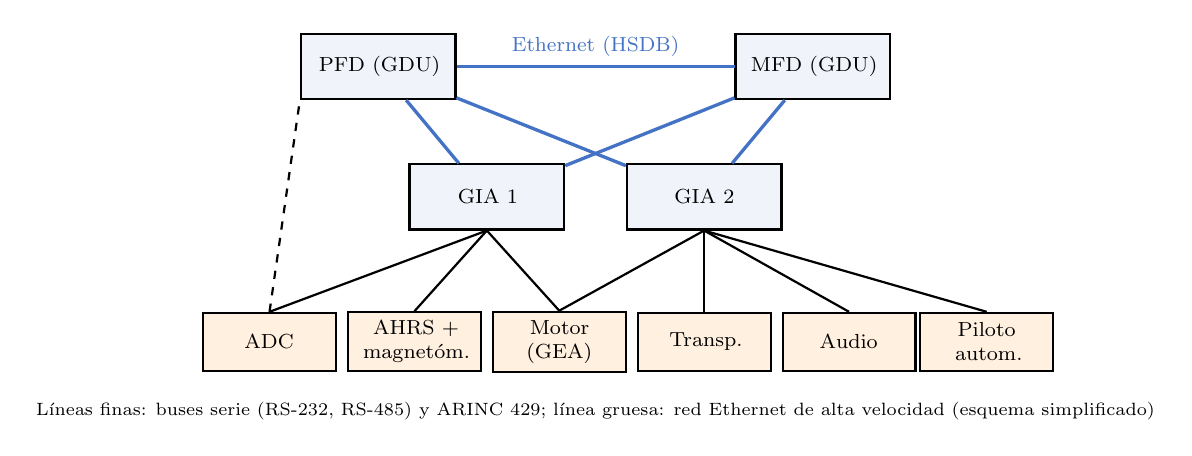
\begin{tikzpicture}[scale=0.92, transform shape, node distance=0.5cm, every node/.style={font=\footnotesize, align=center},
  b/.style={draw, thick, fill=ppAzul!8, minimum height=0.9cm, text width=1.9cm},
  s/.style={draw, thick, fill=orange!12, minimum height=0.8cm, text width=1.6cm}]
  \node[b] (pfd) at (0,3) {PFD (GDU)};
  \node[b] (mfd) at (6,3) {MFD (GDU)};
  \node[b] (g1) at (1.5,1.2) {GIA 1};
  \node[b] (g2) at (4.5,1.2) {GIA 2};
  \draw[very thick, ppAzul] (pfd) -- node[above] {Ethernet (HSDB)} (mfd);
  \draw[very thick, ppAzul] (pfd) -- (g1); \draw[very thick, ppAzul] (mfd) -- (g2);
  \draw[very thick, ppAzul] (pfd) -- (g2); \draw[very thick, ppAzul] (mfd) -- (g1);
  \node[s] (adc) at (-1.5,-0.8) {ADC};
  \node[s] (ahrs) at (0.5,-0.8) {AHRS + magnetóm.};
  \node[s] (gea) at (2.5,-0.8) {Motor (GEA)};
  \node[s] (xpdr) at (4.5,-0.8) {Transp.};
  \node[s] (aud) at (6.5,-0.8) {Audio};
  \node[s] (ap) at (8.4,-0.8) {Piloto autom.};
  \foreach \n in {adc,ahrs,gea} \draw[thick] (\n.north) -- (g1.south);
  \foreach \n in {gea,xpdr,aud,ap} \draw[thick] (\n.north) -- (g2.south);
  \draw[thick, dashed] (adc.north) -- (pfd.south west);
  \node at (3,-1.75) {\scriptsize Líneas finas: buses serie (RS-232, RS-485) y ARINC 429; línea
  gruesa: red Ethernet de alta velocidad (esquema simplificado)};
\end{tikzpicture}
\end{center}

Las pantallas y las GIA forman una red de alta velocidad. Los sensores y equipos periféricos se
conectan, generalmente de forma redundante, a las GIA y a las pantallas mediante buses serie y
ARINC 429. Si se pierde una GIA, el sistema sigue funcionando con la otra (con una radio y un GPS
menos).

% ------------------------------------------------------------
\section*{2. CONFIGURACIÓN, SOFTWARE Y BASES DE DATOS}

\begin{itemize}
  \item \textbf{Modo de configuración:} se ingresa encendiendo las pantallas con una tecla
        presionada (según el procedimiento del fabricante). Permite ver el estado de cada unidad,
        cargar software y configuración, calibrar sensores y leer registros de fallas.
  \item \textbf{Software y configuración:} se cargan desde una \textbf{tarjeta SD} preparada con la
        versión aprobada para esa aeronave. Cuando se reemplaza una unidad (LRU), hay que cargarle
        el software y la configuración correspondientes; si no coinciden, el sistema muestra
        alertas de incompatibilidad.
  \item \textbf{Bases de datos:} navegación (ciclo \textbf{AIRAC} de 28 días), terreno, obstáculos,
        planos de aeropuertos y cartas. Se actualizan por tarjeta SD o en forma inalámbrica en los
        sistemas nuevos. Volar IFR con una base de navegación vencida tiene limitaciones.
  \item \textbf{Registro:} toda carga de software o de configuración se registra en los registros
        de mantenimiento con la versión instalada.
\end{itemize}

% ------------------------------------------------------------
\section*{3. LA FAMILIA G3000 Y G5000}

Para aviones turbohélice y jets, Garmin desarrolló sistemas con pantallas más grandes y
\textbf{controladores táctiles}:
\begin{itemize}
  \item \textbf{G3000:} jets livianos y turbohélices (por ejemplo, HondaJet, Cessna Citation M2 y
        derivados en otros fabricantes).
  \item \textbf{G5000:} jets medianos, como los Cessna Citation Latitude, Longitude y Sovereign+ y
        los Learjet 70/75. Tres pantallas de gran tamaño (14 pulgadas) en formato apaisado, que se
        pueden dividir en ventanas, y \textbf{controladores con pantalla táctil} en el pedestal desde
        donde se manejan radios, plan de vuelo, sistemas y listas de chequeo.
  \item Integran funciones de aviones de transporte: piloto automático con acelerador automático en
        algunos modelos, sistema de alertas de la tripulación (CAS), páginas sinópticas de los
        sistemas (combustible, eléctrico, presurización) y planificación del rendimiento.
  \item Las versiones \textbf{Prime} recientes renovaron el software y la presentación, y aportaron
        funciones que luego se trasladaron a la aviación general.
\end{itemize}

% ------------------------------------------------------------
\section*{4. MANTENIMIENTO DE UN SISTEMA INTEGRADO}
\begin{itemize}
  \item Leer los \textbf{registros de fallas} y las páginas de estado antes de cambiar nada.
  \item Verificar primero \textbf{alimentación, conectores y cableado}: muchas fallas
        ``electrónicas'' son pines flojos, conectores mal asentados o masas deficientes.
  \item Al reemplazar una unidad: anotar número de parte, serie y versión de software; cargar
        software y configuración; realizar las calibraciones y ensayos que indica el manual (por
        ejemplo, AHRS y magnetómetro después de cambiar el AHRS o el magnetómetro).
  \item Ventilación: las pantallas tienen ventiladores; uno trabado provoca sobretemperatura y
        apagado.
  \item Actualizar las bases de datos y registrar la vigencia.
  \item Inspeccionar periódicamente las baterías de reserva y su prueba de capacidad.
\end{itemize}

% ------------------------------------------------------------
\section*{5. ACTIVIDADES DE LA UNIDAD}
\begin{enumerate}
  \item Dibujar el diagrama de interconexión de un G1000 de un Cessna 172 a partir del manual de
        mantenimiento del avión (capítulo 34 o 42, según el fabricante).
  \item ¿Qué funciones se pierden si falla la GIA 1? ¿Y si falla el GDC 74?
  \item Explicar el procedimiento para actualizar la base de datos de navegación y cómo se registra.
  \item Practicar con un entrenador o simulador de G1000 la carga de un plan de vuelo y la lectura
        de las páginas de motor.
  \item Comparar la cabina de un Cessna 172 con G1000 y la de una Citation Latitude con G5000:
        cantidad y tamaño de pantallas, forma de control, funciones.
\end{enumerate}
       % Unidad 4: sistemas integrados G1000 y G5000
% ============================================================
% UNIDAD 5: EQUIPOS DE REEMPLAZO (RETROFIT)
% ============================================================
\clearpage
\section*{UNIDAD 5: EQUIPOS DE REEMPLAZO}
\subsection*{G5, GI 275, G3X Touch, G500/G600 TXi, AXIS y Aspen}

\begin{recuadro}
\textbf{Objetivo de la unidad:} conocer los instrumentos digitales que se instalan para
modernizar aeronaves existentes, sus componentes y sensores, su forma de instalación y sus
diferencias, para poder recomendarlos, instalarlos y mantenerlos.
\end{recuadro}

% ------------------------------------------------------------
\section*{1. POR QUÉ MODERNIZAR UN PANEL}

La mayoría de los aviones de la aviación general argentina tienen décadas de antigüedad e
instrumentos de vacío. Reemplazarlos por instrumentos digitales: elimina la bomba de vacío (una de
las fallas más comunes y peligrosas en vuelo por instrumentos); mejora la confiabilidad; agrega
funciones (HSI con GPS, alertas, motor digital, ADS-B); y aumenta el valor de la aeronave. Los
equipos de reemplazo están pensados para \textbf{instalarse en los orificios existentes} del panel
o con modificaciones mínimas, mediante un STC que cubre muchos modelos.

% ------------------------------------------------------------
\section*{2. INSTRUMENTOS AUTÓNOMOS}

\subsubsection*{2.1. Garmin G5}
\begin{itemize}
  \item Pantalla de 3,5 pulgadas que se monta en un \textbf{orificio estándar de 3 1/8 pulgadas}.
  \item Contiene \textbf{AHRS y ADC internos}: se conecta a las líneas pitot y estática.
  \item Puede configurarse como \textbf{indicador de actitud} (con velocidad y altitud en cintas) o
        como \textbf{indicador de rumbo / HSI} (con el magnetómetro remoto GMU 11 y, para mostrar
        la navegación de un GPS o NAV existente, un adaptador GAD 29).
  \item \textbf{Batería de respaldo} interna: sigue funcionando si se pierde la alimentación.
  \item En aeronaves certificadas se instala por STC como reemplazo del horizonte artificial y del
        indicador de rumbo; también se usa como \textbf{instrumento de reserva} en paneles más
        grandes. Hay una versión experimental para aeronaves amateur y LSA.
  \item Se integra con el piloto automático GFC 500.
\end{itemize}

\subsubsection*{2.2. Garmin GI 275}
\begin{itemize}
  \item También se instala en un orificio de 3 1/8 pulgadas, con pantalla táctil y perilla.
  \item Según la versión y la configuración reemplaza: \textbf{horizonte (ADI)}, \textbf{HSI},
        \textbf{CDI}, \textbf{indicadores de motor (EIS)} o funciona como \textbf{pequeño MFD}
        (mapa, tránsito, meteorología).
  \item La versión ADI tiene AHRS y ADC internos; puede tener batería de respaldo.
  \item Permite reemplazar instrumento por instrumento manteniendo el formato del panel, y es
        compatible con muchos pilotos automáticos antiguos.
\end{itemize}

\subsubsection*{2.3. Aspen Evolution (EFD 1000 PFD)}
\begin{itemize}
  \item Pantalla vertical de 6 pulgadas que ocupa el lugar del \textbf{horizonte y del indicador de
        rumbo}, montada sobre los dos orificios existentes: se instala con muy poca modificación
        del panel.
  \item PFD completo (actitud, cintas de velocidad y altitud, HSI) con sensores internos y un
        \textbf{módulo de sensores remoto (RSM)} montado en el fuselaje (magnetómetro y temperatura).
  \item Batería interna de respaldo. Se conecta a navegadores GPS y radios existentes.
  \item Se complementa con una o dos pantallas MFD de la misma familia.
\end{itemize}

% ------------------------------------------------------------
\section*{3. SISTEMAS DE PANTALLAS}

\subsubsection*{3.1. Garmin G3X Touch}
\begin{itemize}
  \item Pantallas táctiles de 7 y 10,6 pulgadas, configurables como PFD, MFD o ambos.
  \item Sensores remotos: \textbf{ADAHRS} (GSU 25), magnetómetro (GMU 11), sonda de temperatura,
        unidad de motor (GEA 24); se comunican por un \textbf{bus CAN}.
  \item Nació para aeronaves experimentales y LSA; luego se aprobó por STC para muchos modelos
        certificados. Se combina con el G5 como reserva y con el piloto automático GFC 500.
\end{itemize}

\subsubsection*{3.2. Garmin G500 / G600 TXi}
\begin{itemize}
  \item Pantallas táctiles (10,6 y 7 pulgadas) para aeronaves certificadas, en formato horizontal
        o vertical. PFD, MFD e indicación de motor opcional.
  \item Trabajan junto a los navegadores GPS de la familia GTN y radios externas, que siguen en la
        columna central del panel.
\end{itemize}

\subsubsection*{3.3. Garmin AXIS}
\begin{itemize}
  \item Familia de pantallas presentada por Garmin en julio de 2026 para aviones con motor a pistón
        (monomotores y bimotores livianos), mediante un STC con lista de modelos, y para aeronaves
        experimentales y LSA.
  \item Su característica principal es que la pantalla \textbf{integra el navegador GPS IFR, las
        radios de comunicaciones y navegación y el panel de audio}: se elimina la columna central de
        equipos, como en un G1000, pero como modernización.
  \item Comparte muchos sensores, unidades remotas, recortes del panel y agujeros de montaje con el
        G3X Touch, lo que facilita la actualización desde ese sistema.
  \item Agrega conectividad inalámbrica (Bluetooth y Wi-Fi) para bases de datos y planes de vuelo.
\end{itemize}

% ------------------------------------------------------------
\section*{4. CUADRO COMPARATIVO}
\begin{center}
\footnotesize
\begin{tabular}{|>{\raggedright\arraybackslash}p{0.13\linewidth}|>{\raggedright\arraybackslash}p{0.19\linewidth}|>{\raggedright\arraybackslash}p{0.21\linewidth}|>{\raggedright\arraybackslash}p{0.15\linewidth}|>{\raggedright\arraybackslash}p{0.16\linewidth}|}
\hline
\textbf{Equipo} & \textbf{Tipo} & \textbf{Instalación} & \textbf{Sensores} & \textbf{Uso típico} \\
\hline
G5 & Instrumento autónomo & Orificio de 3 1/8 pulg. & Internos + GMU 11 & Reemplazo de vacío;
reserva \\ \hline
GI 275 & Instrumento autónomo multifunción & Orificio de 3 1/8 pulg. & Internos (ADI) & Reemplazo
gradual, motor \\ \hline
Aspen EFD 1000 & PFD autónomo & Dos orificios (horizonte y rumbo) & Internos + RSM & PFD con
poca obra \\ \hline
G3X Touch & Sistema de pantallas & Recorte del panel & ADAHRS remoto, CAN & Experimental, LSA y
certificados \\ \hline
G500/G600 TXi & Sistema de pantallas & Recorte del panel & ADAHRS remoto & Certificados con
columna de radios \\ \hline
AXIS & Pantallas con radios integradas & Recorte del panel & Remotos (familia G3X) & Panel
completo nuevo \\ \hline
\end{tabular}
\end{center}
Otras marcas presentes en el mercado: Dynon (SkyView, con versiones certificadas por STC), uAvionix
(AV-30), Avidyne, MGL y otras. El criterio de elección incluye: aeronave y su STC, uso (VFR o IFR),
piloto automático, presupuesto, peso, consumo eléctrico y soporte técnico disponible en el país.

% ------------------------------------------------------------
\section*{5. ACTIVIDADES DE LA UNIDAD}
\begin{enumerate}
  \item Proponer dos alternativas de modernización para un Cessna 172 de 1978 con instrumentos de
        vacío, una económica y una completa, con un esquema del panel resultante.
  \item Leer el manual de instalación del G5 y listar: conexiones eléctricas, conexiones de pitot y
        estática, requisitos del magnetómetro y calibraciones necesarias.
  \item Comparar el diagrama de interconexión de un G3X Touch con el de un G1000: ¿qué buses usa
        cada uno?
  \item Investigar qué equipos de esta unidad tienen STC aceptado por la ANAC y cómo se tramita
        esa aceptación.
\end{enumerate}
    % Unidad 5: G5, GI 275, G3X Touch, TXi, AXIS, Aspen
% ============================================================
% UNIDAD 6: CABLES AERONÁUTICOS, MAZOS Y EWIS
% ============================================================
\clearpage
\section*{UNIDAD 6: CABLES AERONÁUTICOS}
\subsection*{Tipos de cable, selección, mazos, blindajes, masas y EWIS}

\begin{recuadro}
\textbf{Objetivo de la unidad:} conocer los tipos de cables usados en aeronaves, seleccionar la
sección adecuada, armar e instalar mazos según las prácticas aceptadas, y aplicar correctamente
los blindajes y las masas.
\end{recuadro}

% ------------------------------------------------------------
\section*{1. POR QUÉ NO CUALQUIER CABLE}

En una aeronave los cables soportan vibración, temperaturas extremas, fluidos (combustible,
aceite, fluido hidráulico) y, en caso de incendio, no deben propagar la llama ni producir humo
tóxico. Por eso se usan cables con normas específicas. \textbf{Nunca se usan cables con aislación
de PVC} (los de uso domiciliario o automotor): emiten gases tóxicos y corrosivos al quemarse.

El conjunto de cables, conectores, terminales, soportes y protecciones de una aeronave se denomina
\textbf{EWIS} (\textit{Electrical Wiring Interconnection System}). Después de accidentes como el
del TWA 800 (1996) y el Swissair 111 (1998), en los que el cableado fue protagonista, las
autoridades reforzaron los requisitos de diseño, inspección y mantenimiento del cableado.

% ------------------------------------------------------------
\section*{2. TIPOS DE CABLES}

\begin{center}
\small
\begin{tabular}{|p{0.28\linewidth}|p{0.34\linewidth}|p{0.26\linewidth}|}
\hline
\textbf{Norma} & \textbf{Características} & \textbf{Uso} \\ \hline
SAE AS22759 (ex MIL-W-22759) /16, /32, /34 & Conductor de cobre estañado, aislación de ETFE
(Tefzel) o ETFE reticulado; 600 V; hasta 150 $^\circ$C. & El más usado en aviónica de aviación
general \\ \hline
AS22759 con conductor plateado o niquelado & Mayor temperatura (200 $^\circ$C o más). & Zonas
calientes, motor \\ \hline
MIL-W-81381 (poliimida, ``Kapton'') & Muy delgado y liviano, pero se fisura y puede producir
\textbf{arcos que se propagan} (\textit{arc tracking}). & Aeronaves antiguas; hoy se evita y se
inspecciona con cuidado \\ \hline
M27500 & Cable multiconductor con o sin \textbf{blindaje} y cubierta, armado con conductores
AS22759. & Señales, audio, buses de datos \\ \hline
Coaxiales M17 (RG-400, RG-142) & 50 $\Omega$, PTFE. & Antenas (Unidad de microondas) \\ \hline
Cables de par trenzado especiales & Impedancia controlada (por ejemplo, para Ethernet o buses de
datos). & Redes de aviónica \\ \hline
\end{tabular}
\end{center}

\paragraph*{Cómo se lee una designación.} Por ejemplo, \texttt{M22759/16-22-9}: norma 22759,
hoja de especificación 16 (ETFE, cobre estañado), sección \textbf{22 AWG}, color \textbf{9}
(blanco). Un M27500 lleva en su designación la cantidad de conductores, su tipo, el blindaje y la
cubierta.

% ------------------------------------------------------------
\section*{3. SELECCIÓN DE LA SECCIÓN (AWG)}

La sección del cable se elige por dos criterios: que \textbf{no se caliente} (corriente admisible,
según si va solo o en mazo y la altitud) y que la \textbf{caída de tensión} no supere los límites.
Las tablas y gráficos de la circular \textbf{FAA AC 43.13-1B, capítulo 11}, son la referencia
habitual.

\begin{center}
\small
\begin{tabular}{|c|c|c|}
\hline
\textbf{AWG} & \textbf{Resistencia aprox. ($\Omega$ cada 1000 pies)} & \textbf{Uso típico en
aviónica} \\ \hline
24 & 25,7 & Señales, datos (cuando el fabricante lo permite) \\ \hline
22 & 16,1 & Señales, datos, audio, discretas \\ \hline
20 & 10,1 & Alimentación de equipos de bajo consumo \\ \hline
18 & 6,4 & Alimentación de equipos \\ \hline
16 & 4,0 & Alimentación de equipos de mayor consumo \\ \hline
14 & 2,5 & Barras secundarias, luces \\ \hline
12 & 1,6 & Barras, cargas grandes \\ \hline
10 & 1,0 & Alimentaciones principales \\ \hline
\end{tabular}
\end{center}

\paragraph*{Caída de tensión máxima recomendada} (AC 43.13-1B): en sistemas de 14 V, 0,5 V en
servicio continuo y 1 V intermitente; en sistemas de 28 V, 1 V continuo y 2 V intermitente.

\begin{recuadro}
\textbf{Ejemplo.} Una pantalla consume 3 A a 14 V y está a 4 m (13 pies) del disyuntor. El circuito
tiene ida y vuelta (o masa cercana): longitud efectiva $\approx$ 26 pies con cable 22 AWG:
$R = 26 \times 16{,}1 / 1000 = 0{,}42\ \Omega$; $\Delta V = 3 \times 0{,}42 = 1{,}26$ V. Supera los
0,5 V. Con 18 AWG: $R = 26 \times 6{,}4/1000 = 0{,}17\ \Omega$; $\Delta V = 0{,}5$ V. Con 18 AWG
queda justo en el límite; se elige 18 AWG (o 16 si se quiere margen), siempre respetando lo que
indica el manual de instalación del equipo.
\end{recuadro}

% ------------------------------------------------------------
\section*{4. IDENTIFICACIÓN DE LOS CABLES}

Cada cable se identifica con un código (número de circuito, segmento, sección) impreso sobre la
aislación (por láser o por estampado en caliente) o en manguitos termocontraíbles. Según la AC
43.13-1B, la identificación se coloca a intervalos regulares (no más de 15 pulgadas) y cerca de
cada extremo. El código debe coincidir con el \textbf{plano de cableado}: es lo que permite seguir
un circuito años después.

% ------------------------------------------------------------
\section*{5. MAZOS DE CABLES E INSTALACIÓN}

\begin{itemize}
  \item \textbf{Armado en tablero:} el mazo se arma sobre un tablero con el dibujo a escala y clavos
        o soportes que marcan el recorrido, las ramificaciones y las longitudes.
  \item \textbf{Atado:} con \textbf{hilo de atar encerado o de fibra} (nudos de amarre) o con
        precintos aprobados y apretados con la herramienta adecuada (sin cortar dejando filos).
  \item \textbf{Soporte:} \textbf{abrazaderas acolchadas} (tipo MS21919) cada cierta distancia,
        sin apretar ni aplastar los cables.
  \item \textbf{Pasos por estructura:} siempre con \textbf{pasacables} (\textit{grommets}) o
        protectores de borde; nunca un cable apoyado sobre un borde metálico.
  \item \textbf{Radio de curvatura:} no menor a 10 veces el diámetro exterior del cable o mazo mayor
        (con excepciones en los extremos, según la AC 43.13-1B); en coaxiales, el que indique el
        fabricante.
  \item \textbf{Separación:} los cables deben quedar separados de las líneas de combustible,
        aceite, oxígeno y fluidos, y de los comandos de vuelo; los cables de señales sensibles
        (audio, datos, magnetómetro) separados de los de potencia.
  \item \textbf{Holgura de servicio:} dejar suficiente longitud para poder desconectar y reparar
        un conector; evitar tensiones y roces con piezas móviles.
\end{itemize}

% ------------------------------------------------------------
\section*{6. BLINDAJES Y MASAS}

\begin{itemize}
  \item El \textbf{blindaje} (malla alrededor de los conductores) protege las señales de la
        interferencia y evita que los cables irradien.
  \item Se conecta a masa \textbf{donde lo indique el fabricante}: en un extremo (típico en audio,
        para evitar lazos de masa que producen zumbido) o en ambos (típico en buses de datos y RF).
  \item La conexión se hace con un \textbf{manguito de soldadura} (\textit{solder sleeve}) que suelda
        un cable de drenaje a la malla, o terminando la malla en el \textit{backshell} del conector.
        El ``rabo'' (\textit{pigtail}) de masa debe ser lo más corto posible.
  \item \textbf{Masas de alimentación:} cada equipo con su retorno a un punto de masa o a una barra
        de masas, con terminales bien ajustados sobre superficies limpias. Una masa deficiente
        genera fallas intermitentes, ruido y lecturas erróneas de motor.
  \item \textbf{Bonding} (unión eléctrica de la estructura): se mide en miliohms entre el equipo o
        su bandeja y la estructura.
\end{itemize}

% ------------------------------------------------------------
\section*{7. ACTIVIDADES DE LA UNIDAD}
\begin{enumerate}
  \item Interpretar las designaciones: \texttt{M22759/16-20-2} y \texttt{M22759/32-22-9}.
  \item Calcular la sección necesaria para un equipo de 5 A en 28 V a 6 m del disyuntor.
  \item Identificar en muestras de cables cuáles son aptos para uso aeronáutico y cuáles no.
  \item Armar en un tablero un pequeño mazo de tres ramas con atado de hilo y abrazaderas.
  \item Investigar el rol del cableado en el accidente del Swissair 111 y qué cambió después.
\end{enumerate}
      % Unidad 6: cables, mazos y EWIS
% ============================================================
% UNIDAD 7: TERMINALES, EMPALMES, CRIMPADO Y SOLDADURA
% ============================================================
\clearpage
\section*{UNIDAD 7: TERMINALES Y CRIMPADO}
\subsection*{Pelado, terminales, crimpado, inspección y soldadura}

\begin{recuadro}
\textbf{Objetivo de la unidad:} pelar cables sin dañarlos, seleccionar terminales y empalmes,
crimpar con la herramienta correcta, inspeccionar y ensayar el resultado, y terminar blindajes y
conexiones soldadas según las prácticas aeronáuticas.
\end{recuadro}

% ------------------------------------------------------------
\section*{1. EL PELADO}

\begin{itemize}
  \item Usar \textbf{peladoras de precisión} con la cuchilla correspondiente a la sección y al tipo
        de aislación (o peladoras térmicas para aislaciones delgadas). Nunca pelar con alicate o
        cuchillo.
  \item No cortar ni marcar los hilos: un hilo cortado reduce la sección y es un punto de rotura
        por vibración. La norma admite muy pocos hilos dañados, según la sección.
  \item No retorcer los hilos más de lo que ya vienen trenzados; no estañar un cable que se va a
        crimpar.
  \item La longitud de pelado la indica el fabricante del terminal o del contacto.
\end{itemize}

% ------------------------------------------------------------
\section*{2. TERMINALES Y EMPALMES}

\begin{center}
\small
\begin{tabular}{|p{0.26\linewidth}|p{0.62\linewidth}|}
\hline
\textbf{Tipo} & \textbf{Uso} \\ \hline
Terminal de ojal (anillo) & El preferido en aeronaves: no se sale aunque se afloje el tornillo.
Aislado (con color según la sección) o desnudo. Familias aprobadas como MS25036 o PIDG. \\ \hline
Terminal de horquilla & Solo donde el fabricante lo permite; puede salirse si se afloja. \\ \hline
Terminales para cables gruesos & Para cables de batería y arranque: se crimpan con herramientas
hidráulicas. \\ \hline
Empalmes a tope (\textit{butt splices}) & Unen dos cables en reparaciones. Se evitan en zonas de
movimiento y se escalonan en un mazo. \\ \hline
Contactos de conector & Pines y casquillos que se crimpan e insertan en conectores (Unidad 8). \\
\hline
Manguitos de soldadura & Terminación de blindajes y uniones selladas. \\ \hline
\end{tabular}
\end{center}

\paragraph*{Código de colores de los terminales aislados:} rojo para 22--18 AWG, azul para 16--14
AWG y amarillo para 12--10 AWG.

% ------------------------------------------------------------
\section*{3. EL CRIMPADO}

\subsubsection*{3.1. Qué es un buen crimpado}
El crimpado deforma el barril del terminal sobre los hilos hasta formar una unión \textbf{hermética
a los gases}: metal con metal, sin huecos por donde entre humedad que corroa. Es más confiable que
la soldadura ante la vibración, porque no crea una zona rígida donde los hilos se quiebran.

\subsubsection*{3.2. La herramienta correcta}
\begin{itemize}
  \item \textbf{Pinzas de crimpar con trinquete:} no se abren hasta completar el ciclo, lo que
        asegura una presión constante. Cada matriz corresponde a una familia de terminales y a un
        rango de secciones (color).
  \item \textbf{Crimpadoras para contactos de conectores} con norma militar: la \textbf{M22520/1-01}
        (conocida como AF8) para contactos de 12 a 26 AWG y la \textbf{M22520/2-01} (AFM8) para
        contactos pequeños (de 20 AWG y menores). Se usan con un \textbf{posicionador} o
        \textbf{torreta} específico para cada contacto y un \textbf{selector} de la sección del
        cable.
  \item \textbf{Calibración:} las herramientas se verifican periódicamente con calibres
        pasa/no-pasa (\textit{go/no-go}). Una herramienta fuera de calibración produce crimpados
        flojos que pasan la inspección visual.
  \item \textbf{Nunca} usar alicates comunes ni crimpadoras automotrices sin trinquete.
\end{itemize}

\subsubsection*{3.3. Procedimiento}
\begin{enumerate}
  \item Verificar el número de parte del terminal o contacto y la sección del cable.
  \item Seleccionar la herramienta, la matriz o el posicionador y el selector de sección.
  \item Pelar a la longitud indicada.
  \item Insertar el cable hasta que los hilos se vean en la ventana de inspección (o lleguen al
        tope), sin que la aislación entre en el barril.
  \item Crimpar completando el ciclo del trinquete.
  \item Inspeccionar y, en los ensayos de calidad, realizar el ensayo de tracción.
\end{enumerate}

\subsubsection*{3.4. Inspección}
\begin{center}
\small
\begin{tabular}{|p{0.44\linewidth}|p{0.44\linewidth}|}
\hline
\textbf{Correcto} & \textbf{Defectos} \\ \hline
Hilos visibles en la ventana de inspección o al ras del extremo del barril. & Hilos que no llegan
o hilos sueltos fuera del barril. \\ \hline
Aislación cerca del barril, sin entrar en él (pequeña separación visible). & Aislación atrapada
dentro del crimpado o conductor desnudo expuesto. \\ \hline
Marca de la matriz centrada y simétrica. & Crimpado descentrado, barril fisurado o deformado. \\
\hline
El cable no gira ni se desplaza dentro del terminal. & El cable gira o sale al tirar. \\ \hline
\end{tabular}
\end{center}

\paragraph*{Ensayo de tracción.} Sobre muestras crimpadas con la misma herramienta y el mismo lote,
se aplica una fuerza de tracción especificada para cada sección (valores en la norma del
terminal o contacto o en la AC 43.13-1B). El crimpado debe resistirla sin que el cable se salga. Es
la forma objetiva de validar una herramienta y un operador.

% ------------------------------------------------------------
\section*{4. SOLDADURA Y MANGUITOS}

\begin{itemize}
  \item La soldadura se usa en los contactos de soldar de algunos conectores, en placas y en las
        terminaciones de blindaje con \textbf{manguitos de soldadura}.
  \item Estaño con fundente de colofonia no corrosivo; estación de soldado con temperatura
        controlada; limpiar el fundente después.
  \item La unión debe quedar brillante, con el estaño ``mojando'' el conductor y el contacto, sin
        bolitas ni puntas, y sin que el estaño suba por los hilos más allá del contacto (eso los
        vuelve rígidos y se quiebran).
  \item \textbf{Manguitos de soldadura} (familia M83519): tubo termocontraíble con un anillo de
        estaño y fundente en el centro y anillos selladores en los extremos. Con la pistola de calor
        se contrae el tubo, se funde el estaño que une la malla con el cable de drenaje y se sella
        la unión. Se inspecciona que el anillo se haya fundido por completo.
  \item \textbf{Termocontraíbles} de identificación y protección: con la relación de contracción
        adecuada; calentar parejo, sin quemar.
\end{itemize}

% ------------------------------------------------------------
\section*{5. ACTIVIDADES DE LA UNIDAD}
\begin{enumerate}
  \item Pelar 10 cables de 22 AWG con una peladora de precisión e inspeccionarlos con lupa.
  \item Crimpar terminales de ojal de los tres colores y empalmes a tope; inspeccionar y hacer el
        ensayo de tracción.
  \item Crimpar contactos de conector con la M22520/2-01 y su posicionador; inspeccionar.
  \item Terminar el blindaje de un cable M27500 con manguito de soldadura y cable de drenaje.
  \item Verificar una crimpadora con el calibre pasa/no-pasa y registrar el resultado.
\end{enumerate}
    % Unidad 7: terminales, empalmes, crimpado y soldadura
% ============================================================
% UNIDAD 8: CONECTORES MILITARES Y D-SUB
% ============================================================
\clearpage
\section*{UNIDAD 8: CONECTORES}
\subsection*{Circulares militares, D-sub, contactos y accesorios}

\begin{recuadro}
\textbf{Objetivo de la unidad:} reconocer los conectores usados en aviónica, interpretar su
designación, armar conectores con contactos crimpados e insertados, y usar correctamente sus
herramientas y accesorios.
\end{recuadro}

% ------------------------------------------------------------
\section*{1. CONCEPTOS GENERALES}

\begin{itemize}
  \item \textbf{Pin y casquillo:} el contacto macho (\textit{pin}) y el hembra (\textit{socket}).
        Regla de seguridad: el lado que puede quedar \textbf{energizado} al desconectar debe tener
        \textbf{casquillos} (hembras), para que no queden pines con tensión expuestos.
  \item \textbf{Ficha y receptáculo:} la parte que va en el extremo del cable (\textit{plug}) y la
        que va fija en el equipo o en un panel (\textit{receptacle}).
  \item \textbf{Inserto y arreglo de contactos:} la pieza aislante que sostiene los contactos y su
        distribución (cantidad, tamaño y posición).
  \item \textbf{Polarización o clave:} ranuras y chavetas que impiden conectar dos conectores
        iguales cruzados. Los conectores militares tienen varias posiciones de clave (N normal, A,
        B, C\ldots).
  \item \textbf{Contactos de crimpar y de soldar;} contactos \textbf{removibles} (se insertan y
        extraen con herramientas) o fijos.
\end{itemize}

% ------------------------------------------------------------
\section*{2. CONECTORES D-SUB (SUBMINIATURA D)}

Tienen carcasa en forma de D (que asegura la polarización), una o varias filas de contactos y
tornillos de fijación. La norma militar es la \textbf{MIL-DTL-24308}. Son los conectores de la
mayoría de los equipos de aviónica de aviación general (Garmin, Avidyne, Dynon, entre otros),
generalmente en \textbf{alta densidad} y con contactos de crimpar.

\begin{center}
\small
\begin{tabular}{|c|c|c|}
\hline
\textbf{Tamaño de carcasa} & \textbf{Densidad estándar} & \textbf{Alta densidad} \\ \hline
E & DE-9 (9 contactos) & DE-15 (15) \\ \hline
A & DA-15 (15) & DA-26 (26) \\ \hline
B & DB-25 (25) & DB-44 (44) \\ \hline
C & DC-37 (37) & DC-62 (62) \\ \hline
D & DD-50 (50) & DD-78 (78) \\ \hline
\end{tabular}
\end{center}

\begin{itemize}
  \item Los contactos de crimpar se insertan desde atrás hasta que traban y se extraen con una
        herramienta de extracción que libera la traba.
  \item Los contactos de alta densidad son más pequeños y requieren su propia crimpadora o
        posicionador (el que indica el fabricante del equipo).
  \item \textbf{Numeración:} cada contacto tiene su número grabado en el inserto. Al mirar de frente
        el conector macho y el hembra, la numeración queda espejada. En los planos se indica si la
        vista es ``de frente'' (\textit{mating face}) o ``desde atrás'' (\textit{wire side}):
        confundirla es un error clásico.
  \item \textbf{Carcasas traseras} (\textit{backshells}) metálicas para fijar el mazo, dar alivio de
        tensión y conectar el blindaje a masa.
\end{itemize}

% ------------------------------------------------------------
\section*{3. CONECTORES CIRCULARES MILITARES}

\begin{center}
\small
\begin{tabular}{|p{0.22\linewidth}|p{0.30\linewidth}|p{0.36\linewidth}|}
\hline
\textbf{Norma} & \textbf{Acoplamiento} & \textbf{Características y uso} \\ \hline
MIL-DTL-38999 & Serie I y II: bayoneta; Serie III: roscado autotrabante; Serie IV: de traba
rápida & Alta densidad, sellado ambiental, muy usado en aeronaves modernas, sensores y equipos. \\
\hline
MIL-DTL-26482 & Bayoneta & Tamaño reducido, uso general en aviónica. \\ \hline
MIL-DTL-5015 & Roscado & Robusto, para alimentación y cargas grandes; aeronaves antiguas. \\
\hline
MIL-DTL-83723 & Bayoneta o roscado & Aplicaciones aeronáuticas ambientales. \\ \hline
\end{tabular}
\end{center}

\paragraph*{Cómo se lee una designación MIL-DTL-38999.} Ejemplo: \texttt{D38999/26WD35SN}
\begin{center}
\small
\begin{tabular}{|c|p{0.66\linewidth}|}
\hline
\texttt{D38999} & Norma MIL-DTL-38999 \\ \hline
\texttt{/26} & Tipo de pieza: ficha recta de la serie III (otros números identifican receptáculos de
pared, de brida, pasamuros, etc.) \\ \hline
\texttt{W} & Terminación superficial de la carcasa (por ejemplo, cadmio verde oliva) \\ \hline
\texttt{D} & Tamaño de carcasa (letra A a J) \\ \hline
\texttt{35} & Arreglo de inserto (cantidad y tamaño de contactos) \\ \hline
\texttt{S} & Contactos hembra (\textit{socket}); \texttt{P} para macho (\textit{pin}) \\ \hline
\texttt{N} & Posición de clave normal \\ \hline
\end{tabular}
\end{center}

\paragraph*{Tamaños de contactos.} Se identifican por número: 22D, 20, 16, 12 (cuanto menor el
número, mayor el contacto y la corriente que admite). Cada tamaño acepta un rango de secciones de
cable. También hay contactos coaxiales, de fibra óptica y de alta potencia.

% ------------------------------------------------------------
\section*{4. ARMADO DE UN CONECTOR CON CONTACTOS REMOVIBLES}
\begin{enumerate}
  \item Verificar en el plano el número de parte del conector, de los contactos y la asignación de
        cada cable a cada número de contacto (\textit{pinout}).
  \item Pasar por el cable, antes de crimpar, los accesorios traseros: backshell, alivio de
        tensión, termocontraíbles.
  \item Crimpar cada contacto (Unidad 7) e inspeccionarlo.
  \item Insertar cada contacto por la parte trasera del inserto con la \textbf{herramienta de
        inserción} (de plástico, familia M81969/14) hasta escuchar o sentir la traba. Tirar
        suavemente del cable para verificar que quedó trabado.
  \item Colocar \textbf{tapones de sellado} en todas las cavidades sin uso: si quedan abiertas, se
        pierde el sellado ambiental.
  \item Armar el backshell, conectar el blindaje y ajustar al torque indicado.
  \item Verificar \textbf{pin a pin} la continuidad y el aislamiento contra el plano.
\end{enumerate}
Para extraer un contacto se usa la \textbf{herramienta de extracción} del tamaño correcto,
introducida desde atrás (o desde el frente, según el conector) para liberar la traba. Usar la
herramienta equivocada daña el inserto, y entonces hay que cambiar el conector.

\begin{recuadro}
\textbf{Conectores en la aeronave.} Los conectores roscados en zonas de vibración se aseguran con
\textbf{alambre de frenar} o son autotrabantes; los de bayoneta, con su traba. Antes de conectar:
inspeccionar que no haya pines doblados, retraídos o contactos ``empujados'' hacia atrás, suciedad o
humedad. Nunca forzar un conector: si no entra, algo está mal (clave, pin doblado).
\end{recuadro}

% ------------------------------------------------------------
\section*{5. OTROS ELEMENTOS DE INTERCONEXIÓN}
\begin{itemize}
  \item \textbf{Conectores de bandeja} (ARINC 404 y ARINC 600): en los racks de aviónica de los aviones
        de transporte, con contactos de señal, de potencia y coaxiales.
  \item \textbf{Bloques de unión y de masa} (sistemas de módulos con contactos crimpados, familia
        M81714): permiten unir varios cables a un mismo punto (por ejemplo, todas las masas de un
        equipo) sin empalmes.
  \item \textbf{Regletas de terminales} con tornillos: para cables con terminales de ojal.
  \item \textbf{Disyuntores (\textit{circuit breakers})}, interruptores, relés y fusibles (Unidad 9).
\end{itemize}

% ------------------------------------------------------------
\section*{6. ACTIVIDADES DE LA UNIDAD}
\begin{enumerate}
  \item Interpretar las designaciones \texttt{D38999/20WB98PN} y \texttt{D38999/26WJ61SA}
        (usar una tabla de arreglos de insertos).
  \item Armar un conector D-sub de alta densidad de 26 contactos siguiendo un pinout dado.
  \item Insertar y extraer contactos de un conector MIL-DTL-38999 con las herramientas correctas.
  \item Identificar los conectores de un equipo de aviónica real y buscar su número de parte en el
        manual de instalación.
\end{enumerate}
  % Unidad 8: conectores militares y D-sub
% ============================================================
% UNIDAD 9: HERRAMIENTAS Y FERRETERÍA APLICADA A LA AVIÓNICA
% ============================================================
\clearpage
\section*{UNIDAD 9: HERRAMIENTAS Y FERRETERÍA}
\subsection*{Herramental del taller y materiales eléctricos y electrónicos}

\begin{recuadro}
\textbf{Objetivo de la unidad:} conocer, seleccionar y usar correctamente las herramientas e
instrumentos del taller de aviónica, y los elementos de ferretería, materiales y consumibles
eléctricos y electrónicos aprobados para aeronaves.
\end{recuadro}

% ------------------------------------------------------------
\section*{1. HERRAMIENTAS DE CABLEADO}
\begin{center}
\small
\begin{tabular}{|p{0.30\linewidth}|p{0.58\linewidth}|}
\hline
\textbf{Herramienta} & \textbf{Uso y cuidados} \\ \hline
Peladoras de precisión & Con cuchillas para cada sección; no usar con cables de otra aislación. \\
\hline
Peladora térmica & Para aislaciones finas y cables de calibre pequeño. \\ \hline
Pinzas de crimpar con trinquete & Terminales y empalmes; matriz según color. Calibración
periódica. \\ \hline
Crimpadoras M22520/1-01 y /2-01 & Contactos de conectores, con posicionadores y torretas. \\
\hline
Herramientas de inserción y extracción & Una por tamaño de contacto; se reemplazan si se doblan.
\\ \hline
Alicates de corte al ras & Cortes limpios de cables y precintos sin dejar filos. \\ \hline
Herramienta tensora de precintos & Aprieta y corta los precintos a la tensión correcta. \\ \hline
Pistola de calor & Termocontraíbles y manguitos de soldadura, con boquillas reflectoras. \\ \hline
Estación de soldado y desoldado & Con temperatura controlada y punta adecuada. \\ \hline
Tablero de mazos & Para armar los mazos a escala. \\ \hline
Etiquetadora o impresora de manguitos & Identificación de cables. \\ \hline
\end{tabular}
\end{center}

% ------------------------------------------------------------
\section*{2. HERRAMIENTAS MECÁNICAS}
\begin{itemize}
  \item \textbf{Destornilladores} de punta correcta (Phillips, Torx, plana) y en buen estado: una
        punta gastada daña la cabeza del tornillo y el panel.
  \item \textbf{Llaves} de boca, estriadas y tubos en pulgadas.
  \item \textbf{Llaves dinamométricas} (torquímetros) para tornillos, tuercas y conectores, con
        calibración vigente.
  \item \textbf{Pinza para alambre de frenar} y alambre de frenar del diámetro y material
        indicados.
  \item \textbf{Sacabocados de panel} (\textit{panel punch}) para los orificios de 2 1/4 y 3 1/8
        pulgadas de los instrumentos; mechas, avellanadores y limas.
  \item \textbf{Remachadora} y herramientas para tuercas remachables y tuercas con placa
        (\textit{nutplates}).
  \item \textbf{Espejo de inspección, linterna y lupa.}
\end{itemize}

% ------------------------------------------------------------
\section*{3. INSTRUMENTOS DE MEDICIÓN}
\begin{center}
\small
\begin{tabular}{|p{0.30\linewidth}|p{0.58\linewidth}|}
\hline
\textbf{Instrumento} & \textbf{Uso} \\ \hline
Multímetro digital & Tensión, corriente, resistencia, continuidad. \\ \hline
Miliohmímetro & Resistencia de masas y \textit{bonding}. \\ \hline
Medidor de aislamiento & Aislamiento de cables, con la tensión adecuada y \textbf{siempre con los
equipos desconectados}. \\ \hline
Osciloscopio & Señales de datos (ARINC 429, CAN, RS-232), sensores, ruido. \\ \hline
Banco de prueba pitot-estático & Ensayo de pérdidas y verificación de altímetros, velocímetros y
ADC (Unidad 11). \\ \hline
Simuladores de sensores & Década de resistencias, calibrador de termocuplas, generador de pulsos
para simular sensores de motor. \\ \hline
Equipos de prueba de navegación y transpondedor & Generadores de señales de VOR/ILS y de radar
secundario. \\ \hline
\end{tabular}
\end{center}

\paragraph*{Control de herramientas.} En un taller aeronáutico cada herramienta está
\textbf{identificada} y \textbf{controlada}: tableros de sombras o cajas con su lugar marcado, para
que al terminar una tarea se compruebe que no quedó ninguna dentro de la aeronave; y las que
requieren calibración llevan su etiqueta con la fecha de vencimiento.

% ------------------------------------------------------------
\section*{4. FERRETERÍA ELÉCTRICA Y ELECTRÓNICA APLICADA}

\subsubsection*{4.1. Protección de circuitos}
\begin{itemize}
  \item \textbf{Disyuntores (\textit{circuit breakers}):} protegen el \textbf{cable} contra
        sobrecorriente. Se dimensionan según la sección del cable y el consumo del equipo, como
        indica el fabricante. Los de tipo extraíble (\textit{push-pull}) permiten además abrir el
        circuito manualmente.
  \item \textbf{Fusibles:} en algunos circuitos y equipos, con repuestos a bordo según la norma.
  \item \textbf{Limitadores de corriente:} protecciones de barras de alta corriente.
\end{itemize}

\subsubsection*{4.2. Conmutación y control}
\begin{itemize}
  \item \textbf{Interruptores} de palanca y de presión con norma aeronáutica, del amperaje correcto.
  \item \textbf{Relés y contactores:} con diodo de supresión en paralelo con la bobina cuando lo
        indica el plano, para evitar los picos de tensión al desconectarla.
  \item \textbf{Interruptor maestro de aviónica:} desconecta los equipos durante el arranque del
        motor para protegerlos de los transitorios.
\end{itemize}

\subsubsection*{4.3. Ferretería de montaje}
Los tornillos, tuercas y arandelas de una aeronave se identifican por su \textbf{norma (AN, MS,
NAS)}, no por su medida: por ejemplo, tornillos de cabeza fresada MS24694 o de cabeza alomada
MS35206, tuercas autofrenantes AN365 o MS21042, arandelas AN960 y tuercas con placa para fijar
paneles e instrumentos. Se usan siempre los que indica el IPC o el manual de instalación; nunca
ferretería comercial sin identificación.

\subsubsection*{4.4. Materiales y consumibles}
\begin{itemize}
  \item Cables aprobados (Unidad 6), terminales, contactos, empalmes y manguitos.
  \item Termocontraíbles (norma AMS-DTL-23053), manguitos de protección, espirales y fundas
        trenzadas.
  \item Hilo de atar, precintos, abrazaderas acolchadas, pasacables y protectores de borde.
  \item Estaño, fundente y limpiadores aprobados.
  \item Selladores, compuestos para juntas y pastas conductoras, según el manual.
  \item Etiquetas y placas de identificación de los disyuntores e interruptores.
\end{itemize}

\begin{recuadro}
\textbf{Trazabilidad.} Todo material que se instala en una aeronave debe poder rastrearse: se
compra a proveedores confiables con \textbf{certificado de conformidad}, se guarda identificado y,
en el caso de los equipos, con su certificado de liberación (por ejemplo, el 8130-3). Un terminal
o un cable ``sin papeles'' puede ser una \textbf{parte no aprobada} (o falsificada) y no se instala.
\end{recuadro}

% ------------------------------------------------------------
\section*{5. ACTIVIDADES DE LA UNIDAD}
\begin{enumerate}
  \item Hacer el inventario de las herramientas del taller con su función, estado y, si
        corresponde, fecha de calibración.
  \item Armar un tablero de sombras para las herramientas de cableado.
  \item Dimensionar el disyuntor y el cable para un equipo de 2,5 A en 14 V según su manual de
        instalación.
  \item Identificar por su norma una muestra de tornillos, tuercas y arandelas.
  \item Hacer el pedido de materiales (con números de parte) para instalar un G5 en un panel.
\end{enumerate}
 % Unidad 9: herramientas y ferretería aplicada a la aviónica
% ============================================================
% UNIDAD 10: INSTALACIÓN, CONFIGURACIÓN Y DOCUMENTACIÓN
% ============================================================
\clearpage
\section*{UNIDAD 10: INSTALACIÓN DE UN PANEL DIGITAL}
\subsection*{Planificación, tablero, cableado, configuración y documentación}

\begin{recuadro}
\textbf{Objetivo de la unidad:} planificar y ejecutar la instalación de instrumentos digitales:
diseño del panel, planos de cableado, armado del mazo, verificaciones antes de energizar,
configuración, calibración y documentación de la alteración.
\end{recuadro}

% ------------------------------------------------------------
\section*{1. PLANIFICACIÓN}
\begin{enumerate}
  \item \textbf{Verificar la elegibilidad:} que la aeronave esté en la lista del STC y que el STC
        esté aceptado por la autoridad; o, en una experimental, los requisitos aplicables.
  \item \textbf{Reunir la documentación:} manual de instalación del equipo, documentos del STC,
        manual de mantenimiento y de cableado de la aeronave.
  \item \textbf{Análisis de carga eléctrica:} que el alternador y las barras soporten el nuevo
        consumo (y lo que se retira).
  \item \textbf{Peso y balanceo:} calcular el cambio de peso y de centro de gravedad.
  \item \textbf{Lista de materiales} con números de parte, y \textbf{plan de trabajo} con tiempos.
\end{enumerate}

% ------------------------------------------------------------
\section*{2. EL PANEL DE INSTRUMENTOS}
\begin{itemize}
  \item \textbf{Ubicación:} el PFD frente al piloto, dentro de su campo visual primario; el
        instrumento de reserva visible desde la posición del piloto (criterios de la AC 23.1311-1).
  \item \textbf{Recortes:} con plantillas del fabricante; en paneles estructurales, verificar que
        el recorte esté aprobado.
  \item \textbf{Ventilación:} espacio detrás del panel y ventiladores cuando el equipo los exige.
  \item \textbf{Iluminación:} los equipos digitales regulan su brillo automáticamente o desde el
        reóstato del panel; la iluminación de los instrumentos restantes y de las placas debe
        quedar uniforme.
  \item \textbf{Placas y rótulos:} interruptores, disyuntores y limitaciones nuevas, según el STC.
\end{itemize}

% ------------------------------------------------------------
\section*{3. EL PLANO DE CABLEADO}

A partir de los diagramas de interconexión del manual de instalación se dibuja el
\textbf{plano de cableado de la aeronave}: cada cable con su identificación, sección, origen
(conector y número de contacto), destino, blindaje y conexión a masa.

\begin{center}
\small
\begin{tabular}{|c|c|c|c|c|p{0.18\linewidth}|}
\hline
\textbf{Cable} & \textbf{AWG} & \textbf{Desde} & \textbf{Hasta} & \textbf{Blindaje} &
\textbf{Señal} \\ \hline
P1-01 & 22 & J1-1 (equipo) & CB ``PFD'' & -- & Alimentación \\ \hline
P1-02 & 22 & J1-2 & Masa GS1 & -- & Masa \\ \hline
P1-10 & 22 & J1-10 & GMU J1-3 & Sí, un extremo & Datos (RS-485 A) \\ \hline
\ldots & & & & & \\ \hline
\end{tabular}
\end{center}
\textit{(Ejemplo ilustrativo de tabla de cableado; los datos reales salen del manual de
instalación.)}

Herramientas útiles: software de dibujo eléctrico o de diseño de mazos, y planillas de cálculo
para las tablas de cables. El plano final queda en la documentación de la aeronave: es lo que
permitirá a otro técnico reparar el sistema dentro de diez años.

% ------------------------------------------------------------
\section*{4. ARMADO Y VERIFICACIÓN DEL MAZO}
\begin{enumerate}
  \item Armar el mazo en el tablero (Unidad 6), crimpar contactos y terminales (Unidad 7) y armar
        los conectores (Unidad 8).
  \item \textbf{Verificación pin a pin:} con el plano y un multímetro (o un probador de mazos),
        verificar cada conexión: continuidad de cada cable, ausencia de cortocircuitos entre
        cables y contra masa, blindajes conectados donde corresponde.
  \item Instalar el mazo en la aeronave con sus abrazaderas, pasacables y separaciones.
  \item \textbf{Verificación antes de conectar los equipos:} con los conectores de los equipos
        \textbf{desconectados}, energizar y medir que en cada pin de alimentación haya la tensión
        correcta y que no haya tensión donde no debe haberla. Luego desenergizar y conectar los
        equipos. Así se evita quemar un equipo por un error de cableado.
\end{enumerate}

% ------------------------------------------------------------
\section*{5. CONFIGURACIÓN Y CALIBRACIÓN}
\begin{itemize}
  \item \textbf{Software:} cargar la versión aprobada.
  \item \textbf{Configuración de la aeronave:} tipo de aeronave, velocidades y marcas de los arcos
        (según el manual de vuelo), unidades, interfaces (puertos serie, ARINC 429 y su velocidad,
        buses), equipos conectados.
  \item \textbf{Sensores de motor:} tipo de cada sensor, rangos, colores, alertas y calibración de
        combustible (llenando los tanques por etapas y registrando cada punto).
  \item \textbf{Calibración del AHRS:} orientación de montaje y nivelación (cabeceo y alabeo) con la
        aeronave en posición de nivelación.
  \item \textbf{Calibración del magnetómetro:} según el procedimiento del fabricante, generalmente
        girando la aeronave en una zona sin interferencias magnéticas.
  \item \textbf{Bases de datos:} cargar las vigentes.
  \item Guardar una copia de la configuración final.
\end{itemize}

% ------------------------------------------------------------
\section*{6. ENSAYOS Y DOCUMENTACIÓN FINAL}
\begin{itemize}
  \item Ensayos en tierra del manual de instalación: funcionamiento de cada función, interfaces
        con radios, GPS, transpondedor y piloto automático, alertas, modos reversionarios y
        batería de reserva.
  \item \textbf{Ensayo pitot-estático} y de altímetro/transpondedor (Unidad 11).
  \item \textbf{Ensayo de compatibilidad electromagnética:} con todos los sistemas funcionando,
        verificar que el nuevo equipo no interfiera con los existentes (y viceversa), por ejemplo
        transmitiendo con las radios y observando las pantallas y el magnetómetro.
  \item Ensayo en vuelo si el STC o el manual lo requiere.
  \item \textbf{Documentación:} registro de la alteración en los registros de mantenimiento,
        formulario de alteración mayor que exija la autoridad, actualización del peso y balanceo,
        \textbf{suplemento del manual de vuelo}, instrucciones de aeronavegabilidad continuada
        (ICA) y planos de cableado actualizados.
\end{itemize}

% ------------------------------------------------------------
\section*{7. ACTIVIDADES DE LA UNIDAD}
\begin{enumerate}
  \item Hacer el plan completo de instalación de un G5 como horizonte artificial en un Piper PA-28:
        elegibilidad, materiales, carga eléctrica, peso, tiempos.
  \item Dibujar el plano de cableado del G5 con su magnetómetro a partir del manual de instalación.
  \item Diseñar en escala un panel con un G3X Touch de 10 pulgadas, un G5 de reserva, radio y
        transpondedor.
  \item Redactar el registro de mantenimiento de la instalación.
\end{enumerate}
 % Unidad 10: instalación, configuración y documentación
% ============================================================
% UNIDAD 11: ENSAYOS, CALIBRACIÓN Y DIAGNÓSTICO DE FALLAS
% ============================================================
\clearpage
\section*{UNIDAD 11: ENSAYOS Y DIAGNÓSTICO}
\subsection*{Sistema pitot-estático, calibración, chequeo funcional y fallas típicas}

\begin{recuadro}
\textbf{Objetivo de la unidad:} realizar los ensayos funcionales de los instrumentos integrados
instalados en la aeronave, en particular el ensayo del sistema pitot-estático, y diagnosticar las
fallas más frecuentes, registrando el trabajo según los procedimientos aeronáuticos.
\end{recuadro}

% ------------------------------------------------------------
\section*{1. ENSAYO DEL SISTEMA PITOT-ESTÁTICO}

Se realiza con un \textbf{banco de prueba pitot-estático} (manual o automático), que se conecta a
las tomas pitot y estática con adaptadores y permite simular altitudes y velocidades aplicando
vacío y presión de forma controlada.

\subsubsection*{1.1. Precauciones}
\begin{itemize}
  \item Leer el procedimiento del AMM y del fabricante del equipo de prueba.
  \item \textbf{Nunca aplicar presión en el sistema estático ni vacío en el pitot} (salvo lo que
        indique el procedimiento) y respetar las velocidades máximas de cambio: los cambios bruscos
        dañan los sensores y los instrumentos.
  \item Mantener siempre la presión del pitot \textbf{mayor o igual} que la estática.
  \item Tapar las tomas no usadas con los adaptadores del banco y retirarlos todos al terminar (con
        cintas de aviso ``REMOVER ANTES DEL VUELO'').
\end{itemize}

\subsubsection*{1.2. Ensayo de pérdidas}
\begin{itemize}
  \item \textbf{Sistema estático:} en aeronaves no presurizadas, la norma de la FAA (FAR 43,
        apéndice E) indica evacuar el sistema hasta que el altímetro marque unos \textbf{1000 pies
        por encima} de la elevación del lugar; sin seguir bombeando, en \textbf{un minuto} la
        altitud indicada \textbf{no debe bajar más de 100 pies}.
  \item \textbf{Sistema pitot:} se aplica presión hasta una velocidad indicada de prueba y se
        verifica que la pérdida en un tiempo dado no supere lo que indica el manual de la
        aeronave.
  \item Las pérdidas típicas aparecen en mangueras resecas, uniones, drenajes y en los equipos
        recién instalados (conexiones de pitot y estática detrás del panel).
\end{itemize}

\subsubsection*{1.3. Verificación de altímetros, velocímetros y ADC}
Con el banco se llevan los instrumentos a distintos valores (altitudes y velocidades de prueba) y
se comparan con las tolerancias del manual. En los sistemas digitales se verifica también la
\textbf{altitud que el ADC envía al transpondedor} (correlación) y que todas las pantallas indiquen
lo mismo. Las normas de la FAA (FAR 91.411 y 91.413) exigen estos ensayos cada 24 meses calendario
para vuelo IFR en espacio controlado y para el transpondedor; verificar los requisitos de las RAAC
vigentes.

% ------------------------------------------------------------
\section*{2. OTROS CHEQUEOS FUNCIONALES}
\begin{center}
\small
\begin{tabular}{|p{0.26\linewidth}|p{0.62\linewidth}|}
\hline
\textbf{Sistema} & \textbf{Chequeo} \\ \hline
AHRS & Alineación al encender, indicación de actitud con la aeronave nivelada, respuesta a
movimientos, ausencia de banderas. \\ \hline
Rumbo / magnetómetro & Comparación con rumbos conocidos (rosa de los vientos) y con la brújula;
verificación con cargas eléctricas encendidas y apagadas. \\ \hline
Indicación de motor & Simular sensores (década de resistencias, calibrador de termocuplas,
generador de pulsos) y verificar lecturas, colores y alertas. \\ \hline
Combustible & Verificar la indicación en varios niveles de carga y la alerta de combustible
bajo. \\ \hline
Interfaces & Navegación del GPS y del VOR/ILS en el HSI, comandos al piloto automático, altitud al
transpondedor, datos de tránsito y meteorología. \\ \hline
Alimentación & Funcionamiento con la batería de reserva al cortar la alimentación principal; prueba
de capacidad de la batería. \\ \hline
Iluminación y pantallas & Brillo, píxeles defectuosos, ventiladores. \\ \hline
\end{tabular}
\end{center}

% ------------------------------------------------------------
\section*{3. DIAGNÓSTICO DE FALLAS}

\paragraph*{Método.} Leer la falla reportada; reproducirla; revisar los registros y las páginas de
estado del sistema; seguir el procedimiento de aislamiento del fabricante; verificar
\textbf{alimentación, masas, conectores y cableado} antes de cambiar una unidad; reemplazar o
reparar; ensayar; registrar.

\begin{center}
\small
\begin{tabular}{|p{0.36\linewidth}|p{0.52\linewidth}|}
\hline
\textbf{Síntoma} & \textbf{Causas posibles} \\ \hline
Cruz roja en actitud y rumbo & AHRS sin alimentación o sin comunicación; conector; falla del AHRS
\\ \hline
Cruz roja en velocidad, altitud y variómetro & ADC; obstrucción o agua en pitot/estática (con
datos erróneos más que cruz roja); comunicación \\ \hline
Rumbo erróneo que cambia al encender equipos & Magnetómetro afectado por un campo magnético
cercano; calibración \\ \hline
Velocidad o altitud erróneas & Pérdidas, agua u obstrucciones en las líneas; tomas estáticas
dañadas \\ \hline
Indicación de motor errática & Masa del sensor, conector, cable de termocupla dañado o empalmado
con cable común \\ \hline
Pantalla que se reinicia & Caída de tensión en el arranque, mala conexión de alimentación,
sobretemperatura \\ \hline
Mensajes de incompatibilidad de configuración & Unidad reemplazada sin cargar software o
configuración \\ \hline
Sin navegación en el HSI & Configuración de la interfaz (ARINC 429, velocidad), cables A/B
invertidos \\ \hline
\end{tabular}
\end{center}

% ------------------------------------------------------------
\section*{4. REGISTRO DEL TRABAJO}
{\small
\renewcommand{\arraystretch}{1.45}
\begin{tabular}{|p{0.955\linewidth}|}
\hline
\textbf{TARJETA DE TRABAJO -- INSTRUMENTOS INTEGRADOS} \hfill N°: \makebox[2cm]{\dotfill} \\ \hline
Aeronave (matrícula y modelo): \dotfill \quad Fecha: \makebox[3cm]{\dotfill} \\ \hline
Equipo / sistema y referencia del manual: \dotfill \\ \hline
Falla reportada o tarea: \\[0.8cm] \hline
Acciones realizadas: \\[1.1cm] \hline
Unidad removida P/N y S/N: \dotfill \quad Instalada P/N y S/N: \makebox[3.6cm]{\dotfill} \\ \hline
Software y configuración cargados (versión): \dotfill \\ \hline
Ensayos realizados (pitot-estático, funcionales, calibraciones) y resultados: \\[1cm] \hline
Equipos de prueba y vencimiento de calibración: \dotfill \\ \hline
Ejecutó (firma y licencia): \dotfill \quad Inspeccionó: \makebox[4.3cm]{\dotfill} \\ \hline
\end{tabular}
}

% ------------------------------------------------------------
\section*{5. ACTIVIDADES DE LA UNIDAD}
\begin{enumerate}
  \item Realizar con el banco del taller un ensayo de pérdidas del sistema estático de una
        aeronave o de un tablero didáctico, y registrar el resultado.
  \item Verificar un altímetro a varias altitudes de prueba y comparar con las tolerancias.
  \item Simular con una década de resistencias y un calibrador las lecturas de temperatura de
        aceite y de un cilindro, y verificar la indicación.
  \item Resolver tres casos de falla planteados por el docente con el método de diagnóstico y
        completar la tarjeta de trabajo.
\end{enumerate}
    % Unidad 11: ensayos, calibración y diagnóstico de fallas
% ============================================================
% TRABAJOS PRÁCTICOS DE TALLER
% ============================================================
\clearpage
\section*{TRABAJOS PRÁCTICOS DE TALLER}
\subsection*{Prácticas formativas de Instrumentos Integrados}

\begin{recuadro}
\textbf{Normas generales:} trabajar con las herramientas indicadas y devolverlas a su lugar;
registrar cada práctica en la planilla; respetar las normas de seguridad y de ESD; entregar las
piezas realizadas (terminales, conectores, mazos) con la tarjeta de identificación del grupo para
su evaluación.
\end{recuadro}

\subsubsection*{TP 1 -- Pelado y crimpado de terminales}
\textbf{Objetivo:} lograr crimpados aprobables y validarlos.\\
\textbf{Materiales:} cable AS22759 de 22, 18 y 14 AWG, peladora de precisión, terminales de ojal y
empalmes aislados de los tres colores, pinza de trinquete, dinamómetro o banco de tracción, lupa.\\
\textbf{Procedimiento:} pelar y crimpar 5 terminales y 2 empalmes por sección; inspeccionar con lupa
según la tabla de la Unidad 7; ensayar a tracción 2 muestras por sección y registrar la fuerza;
analizar los defectos encontrados.

\subsubsection*{TP 2 -- Contactos de conector y D-sub de alta densidad}
\textbf{Objetivo:} armar un conector D-sub con contactos crimpados según un pinout.\\
\textbf{Materiales:} conector DA-26 de alta densidad con contactos de crimpar, crimpadora y
posicionador adecuados, herramientas de inserción y extracción, backshell, cable multiconductor
blindado.\\
\textbf{Procedimiento:} preparar el cable, crimpar los contactos, insertarlos según el pinout,
colocar el backshell y conectar el blindaje; verificar pin a pin con el multímetro; extraer y volver
a insertar un contacto.

\subsubsection*{TP 3 -- Conector circular MIL-DTL-38999}
\textbf{Objetivo:} manejar contactos removibles de conectores militares.\\
\textbf{Procedimiento:} interpretar la designación del conector y su arreglo de inserto; crimpar
contactos tamaño 22D o 20 con la M22520/2-01 o /1-01 y su posicionador; insertarlos con la
herramienta M81969/14 correspondiente; colocar tapones de sellado en las cavidades libres; armar el
backshell; verificar.

\subsubsection*{TP 4 -- Blindajes y manguitos de soldadura}
\textbf{Objetivo:} terminar correctamente el blindaje de un cable de datos.\\
\textbf{Procedimiento:} pelar la cubierta y peinar la malla según la medida; colocar un manguito de
soldadura con cable de drenaje; contraer con pistola de calor y reflector; inspeccionar la fusión
del anillo de estaño; medir continuidad de la malla al drenaje y aislamiento contra los
conductores.

\subsubsection*{TP 5 -- Mazo de cables en tablero}
\textbf{Objetivo:} construir un mazo real a partir de un plano.\\
\textbf{Procedimiento:} dibujar el tablero a escala 1:1; tender los cables identificados; atar con
hilo encerado; armar conectores y terminales; verificar pin a pin con la tabla de cableado; colocar
manguitos y protecciones; registrar el ensayo.

\subsubsection*{TP 6 -- Configuración y calibración}
\textbf{Objetivo:} recorrer el modo de configuración de un equipo integrado.\\
\textbf{Procedimiento:} con un equipo real en banco (o con el simulador o entrenador del
fabricante), ingresar al modo de configuración, cargar las velocidades y arcos de una aeronave dada,
configurar los sensores de motor y simular sus valores; realizar la calibración de nivelación del
AHRS; guardar la configuración y documentar los pasos.

\subsubsection*{TP 7 -- Ensayo pitot-estático}
\textbf{Objetivo:} realizar un ensayo de pérdidas y de indicación.\\
\textbf{Procedimiento:} conectar el banco al sistema de la aeronave o a un tablero didáctico;
realizar el ensayo de pérdidas del sistema estático y del pitot; verificar un altímetro y un
velocímetro en varios puntos; comparar con las tolerancias; completar la tarjeta de trabajo.

\subsubsection*{TP 8 -- Diagnóstico de fallas}
\textbf{Objetivo:} aplicar el método de diagnóstico.\\
\textbf{Procedimiento:} el docente introduce fallas en el tablero didáctico (contacto retraído,
masa abierta, cables A/B invertidos, blindaje cortado, pérdida en una manguera); cada grupo las
diagnostica con el plano, el multímetro y el banco, las corrige y documenta.

\subsubsection*{Formato del informe}
Carátula; objetivo; herramientas y materiales (con números de parte); procedimiento; mediciones y
resultados; fotografías de las piezas realizadas; defectos encontrados y su corrección;
conclusiones sobre la aplicación en el trabajo real.
      % Trabajos prácticos de taller
% ============================================================
% PROYECTO INTEGRADOR: PANEL DIDÁCTICO CON MAZO DE CABLES
% ============================================================
\clearpage
\section*{PROYECTO INTEGRADOR}
\subsection*{Panel de instrumentos didáctico con su mazo de cables}

\begin{recuadro}
\textbf{Consigna general:} diseñar y construir un \textbf{panel de instrumentos didáctico} para el
taller, con instrumentos digitales reales o simulados, su mazo de cables completo hecho con
materiales y técnicas aeronáuticas, y toda la documentación de una instalación real.

\textbf{Modalidad:} grupos de cuatro o cinco estudiantes. \textbf{Entrega final:} panel funcionando,
carpeta técnica y presentación oral.
\end{recuadro}

% ------------------------------------------------------------
\section*{1. ALCANCE}
El grupo elige una de estas opciones según el equipamiento disponible:
\begin{itemize}
  \item \textbf{Opción A -- Equipos reales:} panel con un instrumento digital (G5, GI 275 o
        similar), su magnetómetro y, si se dispone, un transpondedor o radio, cableados según el
        manual de instalación del fabricante, con líneas pitot y estática para ensayarlo con el
        banco.
  \item \textbf{Opción B -- Instrumento digital de construcción propia:} un ``EFIS didáctico''
        hecho con un microcontrolador (por ejemplo, ESP32), un sensor de giróscopos y
        acelerómetros, un sensor de presión barométrica y una pantalla, que muestre actitud,
        altitud y velocidad vertical. Se cablea con conectores D-sub y circulares, cables
        aeronáuticos y un disyuntor, como si fuera un equipo certificado.
  \item \textbf{Opción C -- Mazo de instalación completo:} el mazo de cables para la instalación de
        un sistema real (por ejemplo, un G3X Touch con sus sensores), construido a partir de los
        diagramas del manual de instalación, con cajas que simulan cada equipo y sus conectores.
\end{itemize}

% ------------------------------------------------------------
\section*{2. ETAPAS}
\begin{center}
\small
\begin{tabular}{|c|p{0.62\linewidth}|c|}
\hline
\textbf{Etapa} & \textbf{Tareas} & \textbf{Semanas} \\ \hline
1 & Estudio del manual de instalación; lista de materiales con números de parte; análisis de
carga eléctrica. & 2 \\ \hline
2 & Diseño del panel (escala 1:1), plano de cableado y tabla de cables. & 3 \\ \hline
3 & Construcción del panel: recortes, montaje, placas e iluminación. & 2 \\ \hline
4 & Armado del mazo en tablero: crimpado, conectores, blindajes, identificación. & 4 \\ \hline
5 & Verificación pin a pin y verificación de tensiones antes de conectar los equipos. & 1 \\ \hline
6 & Configuración, calibración y ensayos funcionales (y pitot-estático, en la opción A). & 2 \\
\hline
7 & Carpeta técnica, registros e instrucciones de mantenimiento; presentación oral. & 2 \\ \hline
\end{tabular}
\end{center}

% ------------------------------------------------------------
\section*{3. CARPETA TÉCNICA}
\begin{enumerate}
  \item Descripción del sistema y diagrama de bloques.
  \item Lista de materiales con números de parte y certificados de los materiales usados.
  \item Plano del panel y plano de cableado con su tabla de cables.
  \item Registros de inspección de crimpados y ensayos de tracción.
  \item Planilla de verificación pin a pin y de tensiones.
  \item Configuración del equipo y registros de calibración.
  \item Resultados de los ensayos funcionales.
  \item Instrucciones de mantenimiento del panel y tarjeta de trabajo.
\end{enumerate}

% ------------------------------------------------------------
\section*{4. EVALUACIÓN}
\begin{center}
\small
\begin{tabular}{|p{0.66\linewidth}|c|}
\hline
\textbf{Criterio} & \textbf{Peso} \\ \hline
Diseño: plano del panel, plano de cableado y lista de materiales & 20\% \\ \hline
Calidad del mazo: crimpados, conectores, blindajes, atado e identificación & 30\% \\ \hline
Verificaciones y ensayos realizados y documentados & 20\% \\ \hline
Funcionamiento del panel & 15\% \\ \hline
Carpeta técnica y presentación oral & 15\% \\ \hline
\end{tabular}
\end{center}

\begin{recuadro}
\textbf{Para el CV:} \textit{``Diseño y construcción de un panel de instrumentos digitales con su
mazo de cables según prácticas aeronáuticas (AC 43.13-1B): crimpado con herramientas M22520,
conectores MIL-DTL-38999 y D-sub, blindajes, verificación pin a pin, configuración y ensayos''}.
\end{recuadro}
 % Proyecto integrador: panel didáctico con mazo de cables
\end{document}
